\documentclass[12pt]{witseiepaper}
\usepackage{KJN}
\usepackage[a4paper,top=25mm, bottom=32mm, left=20mm, right=20mm]{geometry}
\usepackage{pdfpages}
% Set the page size to be A4 as opposed to the default US Letter
\usepackage{graphicx} 

% Required for including pictures
\usepackage{float} 


\usepackage{wrapfig} 

%%%%%%%%%%%%%%%
\usepackage{fancyhdr}
\usepackage{pdfpages}

\pagestyle{fancy}
\fancyhf{}
\fancyfoot[C]{\thepage}

\ifpdf
\pdfinfo{
% /Title (INSTRUCTIONS AND STYLE GUIDELINES FOR THE PREPARATION OF FINAL YEAR LABORATORY PROJECT PAPERS : 2005 VERSION)
% /Author (Ken J Nixon)
% /CreationDate (D:200309251200)
% /ModDate (D:200510121530)
% /Subject (ELEN417/455 Paper Format, 2005)
% /Keywords (ELEN417, ELEN455, paper, instructions, style guidelines, laboratory project)
}
\fi

%%%%%%%%%%%%%%%%%%%%%%%%%%%%%%%%%%%%%%%%%%%%%%%%%%%%%%%%%%%%%%%%%%%%%%%%%%%%%%%

\begin{document}


%----------------------------------------------------------------------------------------
% TITLE PAGE
%----------------------------------------------------------------------------------------
\begin{titlepage}
  
  \newcommand{\HRule}{\rule{\linewidth}{0.5mm}} 
  
  % Defines a new command for the horizontal lines, change thickness here
  \begin{center}
    
    % Center everythingn the page
    \textsc{\LARGE ELEN7045}\\[1.5cm]
    
    % Name of your university/college
    \textsc{\Large University of Witwatersrand}\\[0.5cm]
    
    % Major heading such as course name
    \textsc{\large  Group Project Report}\\[0.5cm]
    
    % Minor heading such as course title
    \HRule \\[0.4cm]
    { \huge \bfseries SirVey}\\[0.5cm]
    
    % Title of your document
    \HRule \\[1.5cm]
    \begin{minipage}
      {0.4
      \textwidth} 
      \begin{flushleft}
        \large \emph{Authors:}\\
        Avanindra (Avy) \textsc{Singh} \\
        Leslie \textsc{Dobrowsky} \\
        Lishen \textsc{Ramsudh} \\
        Peter \textsc{Cousins} \\
        Bakwanyana \textsc{Thobela} \\

        
        % Your name
      \end{flushleft}
    \end{minipage}
    ~ 
    \begin{minipage}
      {0.4
      \textwidth} 
      \begin{flushright}
        \large \emph{Student Number:} \\
        0704012 \textsc{N} \\
        9409714 \textsc{M}  \\
        1312875 \\
        782377  \\
        855470
        % Supervisor's Name
      \end{flushright}
    \end{minipage}
    \\[2cm]
    
    {\large \today}\\[2cm]
    
    % Date, change the \today to a set date if you want to be precise
  \end{center}
  \large

 % \textbf{Abstract}  \\[0.1cm]
 %  This document focuses on mock objects. It defines mock objects as a technique in software development commonly used in unit testing. A brief list of when to use mock objects is presented. The differences and a clear definition of each type of ``simulated object'' is given for dummy objects, fake objects, stub objects and mock objects. Mock objects insist on behaviour verification as opposed to other types of objects which usually are state verification. A practical example is illustrated using EasyMock in Java. The application of mock objects in unit testing is then discussed. It is concluded that using mock objects can be a advantage or disadvantage depending on the context of the system under test.

  \textbf{}
  % Dummy text
  %\end{flushleft}
  %\includegraphics{Logo}\\[1cm] % Include a department/university logo - this will require the graphicx package
  %\vfill % Fill the rest of the page with whitespace
\end{titlepage}


% \title{INSTRUCTIONS AND STYLE GUIDELINES FOR THE PREPARATION OF FINAL YEAR LABORATORY PROJECT PAPERS : 2005 VERSION}

% \author{Ken J. Nixon
% \thanks{School of Electrical \& Information Engineering, University of the
% Witwatersrand, Private Bag 3, 2050, Johannesburg, South Africa}
% }

%%%%%%%%%%%%%%%%%%%%%%%%%%%%%%%%%%%%%%%%%%%%%%%%%%%%%%%%%%%%%%%%%%%%%%%%%%%%%%%
%%%%%%%%%%%%%%%%%%%%%%%%%%%%%%%%%%%%%%%%%%%%%%%%%%%%%%%%%%%%%%%%%%%%%%%%%%%%%%%
%%%%%%%%%%%%%%%%%%%%%%%%%%%%%%%%%%%%%%%%%%%%%%%%%%%%%%%%%%%%%%%%%%%%%%%%%%%%%%%'

%----------------------------------------------------------------------------------------
% DECLARATION PAGE
% Your institution may give you a different text to place here
%----------------------------------------------------------------------------------------
 % \renewcommand\thesection{\Alph{section}}
 % \setcounter{section}{0}

 \thispagestyle{empty}\pagestyle{empty}
 \begin{center}
 % \section{DECLARATION}
  \textsc{\bfseries DECLARATION} \\ [1.0cm]
 \end{center}
I ALTER THIS TO PLEDGEARISM AND GROUP WORK BREAKDOWN, Avanindra Singh, declare that this thesis titled, 'My Thesis' and the work presented in it are my own. I confirm that:

\begin{itemize} 
\item This work was done wholly or mainly while in candidature for a research degree at this University. \\
\item Where any part of this thesis has previously been submitted for a degree or any other qualification at this University or any other institution, this has been clearly stated. \\
\item Where I have consulted the published work of others, this is always clearly attributed. \\
\item Where I have quoted from the work of others, the source is always given. With the exception of such quotations, this thesis is entirely my own work. \\
\item I have acknowledged all main sources of help. \\
\item Where the thesis is based on work done by myself jointly with others, I have made clear exactly what was done by others and what I have contributed myself.\\ [1.5cm]
\end{itemize}

% Signed:\\
% \rule[1em]{25em}{0.5pt} % This prints a line for the signature
%  \\ [1.5cm]
% Date:\\
% \rule[1em]{25em}{0.5pt} % This prints a line to write the date



\clearpage % Start a new page

%%%%%%%%%%%%%%%%%%%%%%%%%%%%%%%%%%%%%%%%%%%%%%%%%%%%%%%%%%%%%%%%%%%%%%%%%%%%%%%
%%%%%%%%%%%%%%%%%%%%%%%%%%%%%%%%%%%%%%%%%%%%%%%%%%%%%%%%%%%%%%%%%%%%%%%%%%%%%%%
%%%%%%%%%%%%%%%%%%%%%%%%%%%%%%%%%%%%%%%%%%%%%%%%%%%%%%%%%%%%%%%%%%%%%%%%%%%%%%%

%----------------------------------------------------------------------------------------
% QUOTATION PAGE
%----------------------------------------------------------------------------------------

% \pagestyle{empty} % No headers or footers for the following pages

% \null\vfill % Add some space to move the quote down the page a bit

% \textit{``Thanks to my solid academic training, today I can write hundreds of words on virtually any topic without possessing a shred of information, which is how I got a good job in journalism."}

% \begin{flushright}
% Dave Barry
% \end{flushright}

% \vfill\vfill\vfill\vfill\vfill\vfill\null % Add some space at the bottom to position the quote just right

% \clearpage % Start a new page


%%%%%%%%%%%%%%%%%%%%%%%%%%%%%%%%%%%%%%%%%%%%%%%%%%%%%%%%%%%%%%%%%%%%%%%%%%%%%%%
%%%%%%%%%%%%%%%%%%%%%%%%%%%%%%%%%%%%%%%%%%%%%%%%%%%%%%%%%%%%%%%%%%%%%%%%%%%%%%%
%%%%%%%%%%%%%%%%%%%%%%%%%%%%%%%%%%%%%%%%%%%%%%%%%%%%%%%%%%%%%%%%%%%%%%%%%%%%%%%
%%%%%%%%%%%%%%%%%%%%%%%%%%%%%%%%%%%%%%%%%%%%%%%%%%%%%%%%%%%%%%%%%%%%%%%%%%%%%%%
%%%%%%%%%%%%%%%%%%%%%%%%%%%%%%%%%%%%%%%%%%%%%%%%%%%%%%%%%%%%%%%%%%%%%%%%%%%%%%%
%%%%%%%%%%%%%%%%%%%%%%%%%%%%%%%%%%%%%%%%%%%%%%%%%%%%%%%%%%%%%%%%%%%%%%%%%%%%%%%
 \thispagestyle{empty}\pagestyle{empty}
 \begin{center}
  \textsc{\bfseries ABSTRACT} \\ [1.0cm]
  % \section{ABSTRACT}
  \end{center}
  This document focuses on mock objects. It defines mock objects as a technique in software development commonly used in unit testing. A brief list of when to use mock objects is presented. The differences and a clear definition of each type of ``simulated object'' is given for dummy objects, fake objects, stub objects and mock objects. Mock objects insist on behaviour verification as opposed to other types of objects which usually are state verification. A practical example is illustrated using EasyMock in Java. The application of mock objects in unit testing is then discussed. It is concluded that using mock objects can be a advantage or disadvantage depending on the context of the system under test.
 \\

{\bfseries Key Words: } Software Prototype, Survey, SCRUM .\\ [1.0cm]
% %


\keywords{Four to six key words in alphabetical order, separated by commas.}

\clearpage % Start a new page
%%%%%%%%%%%%%%%%%%%%%%%%%%%%%%%%%%%%%%%%%%%%%%%%%%%%%%%%%%%%%%%%%%%%%%%%%%%%%%%
%%%%%%%%%%%%%%%%%%%%%%%%%%%%%%%%%%%%%%%%%%%%%%%%%%%%%%%%%%%%%%%%%%%%%%%%%%%%%%%
% %%%%%%%%%%%%%%%%%%%%%%%%%%%%%%%%%%%%%%%%%%%%%%%%%%%%%%%%%%%%%%%%%%%%%%%%%%%%%%%
%  \thispagestyle{empty}\pagestyle{empty}
%  \begin{center}
%  % \textsc{\bfseries ACKNOWLEDGEMENTS} \\ [1.0cm]
%  \section{ACKNOWLEDGEMENTS}
%  \end{center}
% The acknowledgements and the people to thank go here, don't forget to include your project advisor.
% The preferred spelling of the word ``acknowledgement'' in British English is
% with an ``e'' after the ``g.'' Use the singular heading even if you have
% several acknowledgements. Use this section for sponsor and financial support
% acknowledgments. This is also an ideal section to acknowledge the
% contribution made by your fellow group member.

% The authors would like to acknowledge the Department of Electronic and
% Electrical Engineering at the University of Sheffield for the use of their
% paper template for the LDIA2003 symposium proceedings as well as the South
% African Institute of Electrical Engineers for parts of the style guidelines
% for publications in the SAIEE transactions.  Additional thanks are extended to
% Andr\'e van Zyl and Steve Levitt for their invaluable contributions.




% \clearpage % Start a new page

% %%%%%%%%%%%%%%%%%%%%%%%%%%%%%%%%%%%%%%%%%%%%%%%%%%%%%%%%%%%%%%%%%%%%%%%%%%%%%%%





%%%%%%%%%%%%%%%%%%%%%%%%%%%%%%%%%%%%%%%%%%%%%%%%%%%%%%%%%%%%%%%%%%%%%%%%%%%%%%%
%%%%%%%%%%%%%%%%%%%%%%%%%%%%%%%%%%%%%%%%%%%%%%%%%%%%%%%%%%%%%%%%%%%%%%%%%%%%%%%
%%%%%%%%%%%%%%%%%%%%%%%%%%%%%%%%%%%%%%%%%%%%%%%%%%%%%%%%%%%%%%%%%%%%%%%%%%%%%%%
%%%%%%%%%%%%%%%%%%%%%%%%%%%%%%%%%%%%%%%%%%%%%%%%%%%%%%%%%%%%%%%%%%%%%%%%%%%%%%%
%%%%%%%%%%%%%%%%%%%%%%%%%%%%%%%%%%%%%%%%%%%%%%%%%%%%%%%%%%%%%%%%%%%%%%%%%%%%%%%
%%%%%%%%%%%%%%%%%%%%%%%%%%%%%%%%%%%%%%%%%%%%%%%%%%%%%%%%%%%%%%%%%%%%%%%%%%%%%%%




%%%%%%%%%%%%%%%%%%%%%%%%%%%%%%%%%%%%%%%%%%%%%%%%%%%%%%%%%%%%%%%%%%%%%%%%%%%%%%%
%%%%%%%%%%%%%%%%%%%%%%%%%%%%%%%%%%%%%%%%%%%%%%%%%%%%%%%%%%%%%%%%%%%%%%%%%%%%%%%
%%%%%%%%%%%%%%%%%%%%%%%%%%%%%%%%%%%%%%%%%%%%%%%%%%%%%%%%%%%%%%%%%%%%%%%%%%%%%%%
% %%%%%%%%%%%%%%%%%%%%%%%%%%%%%%%%%%%%%%%%%%%%%%%%%%%%%%%%%%%%%%%%%%%%%%%%%%%%%%%




%%%%%%%%%%%%%%%%%%%%%%%%%%%%%%%%%%%%%%%%%%%%%%%%%%%%%%%%%%%%%%%%%%%%%%%%%%%%%%%
%%%%%%%%%%%%%%%%%%%%%%%%%%%%%%%%%%%%%%%%%%%%%%%%%%%%%%%%%%%%%%%%%%%%%%%%%%%%%%%
%%%%%%%%%%%%%%%%%%%%%%%%%%%%%%%%%%%%%%%%%%%%%%%%%%%%%%%%%%%%%%%%%%%%%%%%%%%%%%%
%%%%%%%%%%%%%%%%%%%%%%%%%%%%%%%%%%%%%%%%%%%%%%%%%%%%%%%%%%%%%%%%%%%%%%%%%%%%%%%
%%%%%%%%%%%%%%%%%%%%%%%%%%%%%%%%%%%%%%%%%%%%%%%%%%%%%%%%%%%%%%%%%%%%%%%%%%%%%%%
%%%%%%%%%%%%%%%%%%%%%%%%%%%%%%%%%%%%%%%%%%%%%%%%%%%%%%%%%%%%%%%%%%%%%%%%%%%%%%%




%%%%%%%%%%%%%%%%%%%%%%%%%%%%%%%%%%%%%%%%%%%%%%%%%%%%%%%%%%%%%%%%%%%%%%%%%%%%%%%
%%%%%%%%%%%%%%%%%%%%%%%%%%%%%%%%%%%%%%%%%%%%%%%%%%%%%%%%%%%%%%%%%%%%%%%%%%%%%%%
%%%%%%%%%%%%%%%%%%%%%%%%%%%%%%%%%%%%%%%%%%%%%%%%%%%%%%%%%%%%%%%%%%%%%%%%%%%%%%%
% %%%%%%%%%%%%%%%%%%%%%%%%%%%%%%%%%%%%%%%%%%%%%%%%%%%%%%%%%%%%%%%%%%%%%%%%%%%%%%%
% %
% \abstract{The purpose of this document is to provide an easy-to-use
% template/style sheet to enable authors to prepare papers in the correct format
% and style for the final year laboratory project. This document may be
% downloaded from the School of Electrical and Information Engineering web site
% and can be used as a template. To ensure conformity of appearance it is
% essential that these instructions are followed. The abstract should be limited
% to 50-200 words, which should concisely summarise the paper.}

% \keywords{Four to six key words in alphabetical order, separated by commas.}


% \maketitle
% \thispagestyle{empty}\pagestyle{empty}
\pagestyle{plain}

\pagenumbering{roman}

\tableofcontents
% test\index{test}

\newpage
\listoffigures % Write out the List of Figures
\newpage
\listoftables % Write out the List of Tables
\newpage
\renewcommand\thesection{\arabic{section}}
\renewcommand\thesubsection{\thesection.\arabic{subsection}}
 \setcounter{section}{0}
\pagenumbering{arabic}
\setcounter{page}{1}
%%%%%%%%%%%%%%%%%%%%%%%%%%%%%%%%%%%%%%%%%%%%%%%%%%%%%%%%%%%%%%%%%%%%%%%%%%%%%%%
%
\section{Introduction}
In South Africa there are many services such as electricity, water and healthcare which are freely available to citizens or at low cost. The distribution of these basic resources could be defined as "service delivery". This project is aimed at providing a means to monitor service delivery in our country through the usage of a software application to conduct surveys and collect feed back from any citizen who utilises any service in healthcare. In South Africa, it has been publicised in media that healthcare service delivery has an impact on millions of peoples lives including their mortality \cite{InfantsDie}. Obtaining feedback on the health care system is critical to improving all citizens experiences of the health care system.

The requirements of this project is to obtain feed back from the local community utilising the health care systems in order to improve them, specifically through developing a software application which can be used to conduct surveys. By conducting surveys efficiently and through a software application data can be obtained and analysed to provide appropriate reporting on how efficient the service delivery of health care in a particular area. South Africa as a third world country faces unique challenges such as connectivity to the internet \cite{Internet} which imposes challenges from a application development point of view. 

\subsection{Project Requirements}
The purpose of this project is to design a software application which will be used to gather information on the public health care service delivery and provide appropriate reporting. The surveys will be conducted in areas with little internet connectivity. This means that application must cater for capturing data "offline" and then uploaded centrally for reporting.

\section{Literature Review}
\subsection{Existing Solutions}
There is a large number of solutions that exist in the market in terms of software applications which can be used to conduct surveys. Some of the solutions on the market do satisfy the basic project requirements \cite{ReviewSurvey}. SurveyGizmo \cite{SurveyGizmo} is a web application (software as a service) platform which features 28 different customizable possible survey question and answer combinations. This solution satisfies all requirements in particular the off-line capability, custom reporting and developer integration. SurveyMonkey \cite{SurveyMonkey} is similar to SurveyGizmo in that it offers a similar feature set. It also offers the ability to create custom reporting with text analysis. SurveyMonkey also features telephonic surveys where users are able to create surveys and have respondents answer using voice. 

% Pricing options for this stuff means that existing solution is more effective than building your own app ???? 
% Due to Economics of scale therefore pricing lower, verses building specific solution .... Scale is 1 to 1 for client for our POC prototype instead survey monkey supports Every client  Survey features are Customizable price lower due to volume .... 


\subsection{Standards, Regulations and Policy}
Depending on the information that is captured through survey questions there could be standards, regulations and policies which need to be adhered to. An example of this would be in the health care sector where the Act of 1996 (HIPAA) could be applied. The Act of 1996 (HIPAA) is a set of rules to be followed by health plans, doctors, hospitals and other health care providers \cite{HIPAA}. It is essential to adopt the standards for electronic health care transactions and identifiers for providers, health plans, and employers. To date, the implementation of HIPAA standards has increased the use of electronic data interchange \cite{HIPAA}. HIPAA also contains a privacy rule which protects any data gathered from patients in the health care environment. Therefore to comply with HIPAA it essential for any software to have security so that patients are not compromised in terms of the act. Software should comply completely with HIPAA if it is to be used in a health service delivery environment. \\

\section{Project Framework} 

\subsection{Business Case:} 
  
\noindent By conducting surveys, one can identify the misalignment between services required by communities and services rendered by its designated service providers. The result of gathering information about service delivery (in this scenario specifically health care) is that insights and observations can be gained in order to improve service delivery. This could have a variety of impacts including improving people's ability to receive high levels of service and possibly have an impact on their quality of life. Increasing the amount of engagement with the community allows for feedback to be provided to improve service delivery.

\subsection{Scope of the Application:}
The scope of the application progressively changes with each iteration. As an iteration is successful more features and improvements can be added to each version of the project.

\emph{Key Users} 
\begin{itemize}
  \item \textbf{Surveyors:} These are the individuals who will utilise the application to capture surveys and get responses from the community.
  \item \textbf{Administrators:} These are the business owners who define questions and will create surveys and utilise the reporting features of the application to gain insights from the communities responses.
\end{itemize}

\emph{Stakeholders} 
\begin{itemize}
  \item \textbf{Community:} These are the actual people who utilise services and who will provide feedback on the service delivery through the survey project. The community by voicing their concerns and opinions will enjoy improved services (e.g. health care) provided by the service provider based on the feedback gathered.
  \item \textbf{Application Administrators:} Provide administrator services, maintenance and creation of surveys.
  \item \textbf{Surveyors:} Users who conduct surveys through the platform.
  \item \textbf{Development Team:} Responsible for creating and maintaining the platform. 
\end{itemize}


\subsection{Project Requirements}
\subsubsection{Specification By Example}
Specification by Example (SBE) is a collaborative approach where by the team defines requirements and business orientated functional tests for software based on capturing and illustrating requirements using realistic examples. This method is utilised to obtain the specific requirements of the project.
Table ~\ref{tbl:use} shows a list of the specifications by example that are applicable to the project. Appendix A features the detailed requirement specifications artefacts including key examples as well as the specifications by example.

\begin{table}[htb] \caption{Table showing a list of the key examples.} \label{tbl:use} 
    \begin{center}
  \begin{tabular}
    {|c|c|} \hline \textbf{Use} &\textbf{Description}\\
    \textbf{Case} &\\
    \hline 1 &Conducting a Survey\\
    \hline 2 &Reporting\\
    \hline 3 &Offline Mode\\
    \hline 4 &Survey Administration\\
    \hline 5 &User Access\\
    \hline 
  \end{tabular}
      \end{center}
\end{table}

\subsection{Project Constraints}
\begin{itemize}
  \item The project has a time constraint. 
  \item The project does not have unlimited software development resources and each member of the team has different skills. 
  \item The project should be intellectually challenging and must allow for each member of the team to learn new tools, techniques and programming skills.
  \item The project must contain 25\% original source code.
  \item The project solution must be able to function in an environment with little or no connectivity.
\end{itemize}

\subsection{Project Assumptions}
\begin{itemize}
  \item The users specifically the surveyors are honest and do complete surveys and do not fraudulently answer the surveys themselves.
  \item The surveyors do not necessarily have internet connectivity when doing surveys in the community.
  \item The surveyors have the equipment and resources necessary to utilise the project solution in order to conduct surveys in the community.
  \item The data is uploaded to a central point for analysis and reporting. This means that it is not required to generate reporting at the point of surveying.
\end{itemize}


\subsection{Success Criteria}
\subsubsection{For the users}
\begin{itemize}
  \item Surveyors \begin{itemize}
  \item Surveyors are able to capture answers in the form of yes/no questions, free form text and a selection with predefined answers.
  \end{itemize}
    \item Administrators \begin{itemize}
  \item Administrators should be able to create any surveys with the desired answer options.
  \item They should be able to authenticate and login in to the platform.
  \item Administrators should be able to view reporting information on the surveys which have successfully uploaded to the system.
  \end{itemize}

\end{itemize}

\subsubsection{For the project}
\begin{itemize}
  \item The solution must be able to capture surveys in a off-line mode with the ability to upload to a central point for reporting.
  \item Be able to capture surveys on multiple channels and multiple devices.
  \item The device of choice preferably being Android should support as many devices as possible.
  \item Analytics of the data should be centralised.
  \item Surveys are dynamic and can be refreshed in field (given internet connectivity).
  \item There is no custom configuration necessary on any device that the surveyors utilise. This means they can be provisioned in-field.
  \item The system can handle multiple surveyors in the field gathering responses.
  \item The system can also handle multiple types of surveys.
  \item Training guides and development guides should be documented.
\end{itemize}

\subsection{Licensing Requirements}
This project should utilise MIT licenses and free licences where possible.

\section{Project Execution}
A software project's successful execution relies heavily on the project team meeting all desired success criteria defined in the project requirements. To make sure the project team remains on track a specially role is required within the project team, this is commonly known as a software project manager. \cite{SPM}

The project manager role is to manage all of the organizing and planning of a project. This may entail formalizing task allocation and tracking the estimated effort vs. the actual effort expended.
While tracking the team’s effort the budget and cost analysis also needs to be considered as business or sponsors of the prototype project require the PM to report back on progress vs. project budget spent. \cite{ExpertJudgement}

The effective communication to all project stakeholders forms part of the project manager’s base responsibilities. Clearly and regularly communicating the risks, concerns and progress on a project to the appropriate stakeholders, allows for adjustments and decisions to be made in smaller increments thus allowing the team to adapt and remain on track to achieve the project’s goals.

\subsection{Project Methodology}
Project methodologies in the author's opinion should not be dictated but should rather be discussed and adapted to the team's preferences. During the first meeting the team members stated numerous technologies could achieve the business vision and requirements. However this also lead to scope discussions and possible future scope changes as early as the first planning session.

Due to the highly volatile scope discussions within the team the decision to adopt a crafted quality methodology CITE started to present itself as front runner and methodology of choice. The project team agreed that the SCRUM methodology \cite{ExpertJudgement} would be implemented and the role of the project manager would change to be a SCRUM master. \cite{SCUMMaster}

\subsection{Project Team}

With the preferred methodology chosen the team formed to take the key roles required to execute the SCRUM methodology. The three primary roles the team required where the SCRUM Master, Product Owner and technical experts.\\

\begin{figure}[H]
	\center{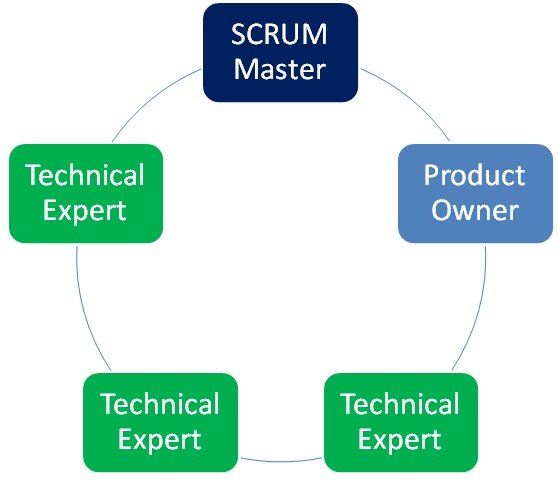
\includegraphics[width=.55\linewidth]{./images/SCRUMTeam}} 
	\caption{SCRUM Team Roles.} 
	\label{fig:SCRUMTeam}
\end{figure}


\subsection{Technology Selection}


\subsection{Sprints}
With the project vision and project deadline defined the high level planning allowed for eleven sprints \cite{ExpertJudgement} where one sprint would run for seven days or 75 effort hours. While de-constructing the requirements the high level deliverables were prioritized in the backlog and marked for delivery in specific sprints. These high level deliverables are shown in figure CITE and the detailed sprint planning can be viewed in appendix C.




\subsection{Project Estimation and Costing}
During the project initiation the business stakeholders will review estimations and high level costing before committing to assigning the budget. The estimations for the proof of concept where based on variable scope and requirements. Due to the variability in requirements the estimation accuracy will not be at a high confidence level. Therefore the POC could result in either an over estimation or under estimating. The proof of concept was estimated at a total of 825 effort hours and 5 resources were assigned, the estimation total was produced using an Expert Judgement method \cite{ExpertJudgement}. The team calculated that a single weekly sprint would consist of 75 hours, this would in turn be the project teams weekly burn rate. Therefore if we assume an average blended resource rate of R 500 an hour the cost per sprint can be calculate as follows.



% MAKE THE TABLE LEFT JUSTIFIED
\begin{table}[htb] \caption{Table showing the effort placed into the project and its cost.} \label{tbl:cost} 
    \begin{center}
  \begin{tabular}
     {|c|c|} %\textbf{Use} &\textbf{Description}\\
    % \textbf{Case} &\\
    \hline Total Project Estimation &825 Hours\\
    \hline Total Sprint Effort Hours &75 Hours\\
    \hline Total Cost per Sprint &R 37 500\\
    \hline Total Cost of POC & R 412 500 \\
    \hline 
  \end{tabular}
      \end{center}
\end{table}

With the POC costing R 412 500 as an estimate the project continued and executed at the required weekly burn rate. However as the requirements become more detailed and clear the project team realized that the estimation had been under quoted. In this scenario depending on the how the contract for this project was drawn up the whether it be a Fixed price or time and materials based contract, would have a direct impact on the teams involved in the project. In the fixed price contract the business stakeholder would pay a single fee regardless of the under or over estimation. The benefit to the software team would be the quicker and cheaper they deliver the working POC the more profit they would make from this software application. If the contract was time and material, specifically with variable requirements the software team will be able to request further funding and the business would need to manage the allocation of additional funding via a formal process (Addition to the Back log, change request or change note).

\subsection{Project Tools}
Various tools were used to enable communication and collaboration within the
group. A high focus was placed on this as the size of the group, distributed resource location, current work commitments, scope changes, technology challenge specifically the learning curve on the chosen technologies all required real time communication to the project team. The tools the team agreed to use are listed in Table CITE.

% MAKE THE TABLE LEFT JUSTIFIED
\begin{table}[htb] \caption{Table showing the tools used by the project team.} \label{tbl:Tools} 
	\begin{center}
		\begin{tabular}
			{|c|c|c|} %\textbf{Use} &\textbf{Description}\\
			% \textbf{Case} &\\
			\hline Communication Tools & Collaboration Tools & Development tools \\
			\hline Weekly Meetings &  Trello Boards & GitHub\\
			\hline Whatsapp & Google Drives &\\
			\hline Phone Calls (Voice) &&\\
			\hline Email &&\\
			\hline 
		\end{tabular}
	\end{center}
\end{table}

Project Communication was implemented via gathering all the contact details for the project team, these were shared and used to create email and a Whatsapp group for real time feedback. Formal Meetings where held weekly to track progress against the sprint planning vs the resource progress and formal meeting minutes where then sent. The formal meeting minutes are detailed in Appendix B. The team Collaboration was controlled by the use of trello boards \cite{Trello} this allowed task assignment, task tracking and progress updates without the need for formal face to face meetings. Managing the developers source code, the development resources agreed to implement GitHub.\cite{GitHubRef} This tool allows the resources to align source code, track changes and backup source code. 

\subsection{Testing}
Testing the project is performed from an acceptance testing level, where the project requirements are directly used to create acceptance tests. \cite{AcceptanceTest} In the context of this project, this level of testing was deemed appropriate as the goal of this project is to identify that the software is capable of achieving the desired client functionality.
The executable specifications produced in the requirement specification are directly utilised in defining the test cases. The advantage noted by executing in this fashion this is that no additional test case creation phase is required at the acceptance level phase and the software is tested using what was jointly agreed upon but all the project stakeholders. The testing is therefore objective in that way.

In terms of the test execution on the project, acceptance tests are run on each of the Sprints in the following manner:



\begin{itemize}
	\item Acceptance testing slots where run at the conclusion of each weekly sprint.
	\item On completion of each specification, the functionality is produced to the project team and is critiqued using the specifications as test cases.
	\item Regression tests are run using specifications to ensure new features do not hamper previously tested functionality.
	\item Failing tests are marked as non-conforming and are re-worked by the developer; re-testing occurs at the next available acceptance testing slot. 
\end{itemize}


%  USER ACCEPTANCE TESTING DONE BY SCRUM TEAM
%  MEETING ALL REQUIREMENTS SPECIFICATIONS BY EXAMPLES 
%  USER TESTING  BAKS STUFF GOES HERE


\section{Engineering the project solution}




\subsection{Overall Architecture}
The project team had created multiple proof of concepts which eventually lead to the final solution which comprises of three major components:
\begin{itemize}
\item Web server 
\item Web client
\item Android application
\end{itemize}

All communication throughout the platform (web server and client components) are executed using RESTful web services provided by the web server. The platform utilises JSON formatting which is a lightweight representation of data based on key value pairs and ordered lists of values \cite{JSON}. Refer to Figure~\ref{fig:Arch} for a diagram of the overall architecture.

\begin{figure}[H]
  \center{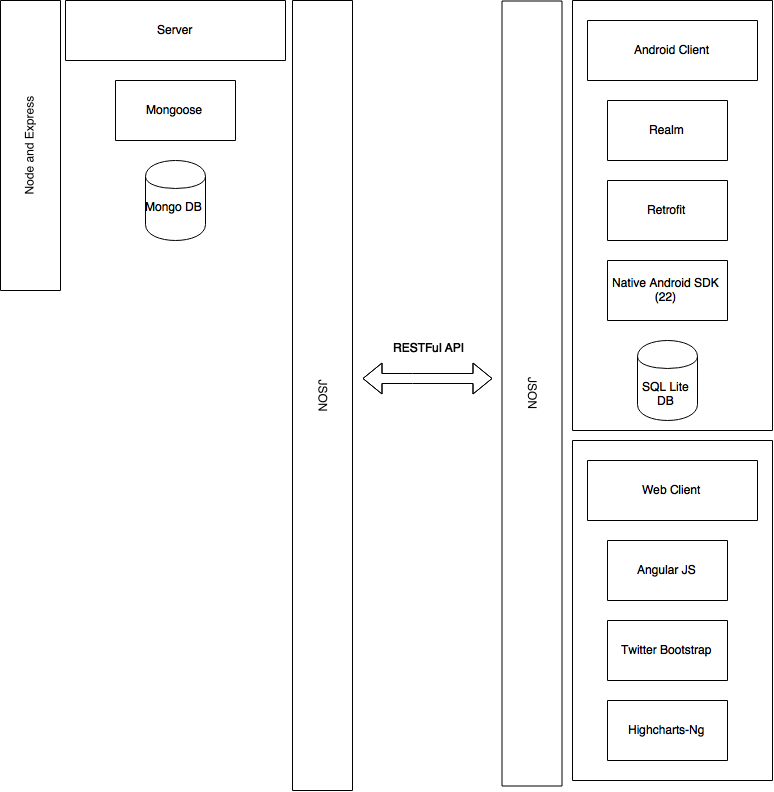
\includegraphics[width=.75\linewidth]{./images/arch.png}} 
  \caption{Proposed Architecture diagram of the system.} 
  \label{fig:Arch}
\end{figure}

The architecture still comprises of the basic 3-tier fundamental framework which follows the Model-View-Controller design pattern. This is present in the web server, web client and android application (adhering to their specific terminology and practices). This complies with the best practices of each of the technologies where given.


\subsection{Web Server}
The web-server is based on a typical client-server communication pattern. The web-based solution is platform independent and 
\subsubsection{Web Server Technology and Design Considerations:} 
The web server utilises a variety of different open source technologies which are all based on Javascript. This allows the entire web stack to be written in one language.

\subsubsection{Technologies used} 
\begin{itemize}
  \item \textbf{MongoDB:} MongoDB is a document based database that utilises a flexible schema \cite{MongoDB}. It stores data in JSON format where each document is a set of key-value pairs that describe the data. Mongo DB is a free and open-source technology.
  \item \textbf{NodeJS:} NodeJS uses Google Chrome's V8 runtime engine to compile javascript on the server on which Node JS is installed and running. It uses an event-driven, non-blocking I/O approach that makes it efficient and lightweight \cite{NodeJS}
  \item \textbf{ExpressJS:} Express JS is a minimal web framework for Node JS applications. It provides libraries that allow the developer to easily develop web solutions using NodeJS \cite{ExpressJS}.
  \item \textbf{Yeoman:} Yeoman allows you to quickly start-up new projects. It prescribes best practices and tools to allow the developer the ability to create applications as quickly as possible \cite{Yeoman}. It makes use of open-source generators to scaffold sections of code that would otherwise be repetitive in nature and take time from building in the business logic which makes up the crux of any application.
  \item \textbf{Angular-Fullstack template from Yeoman:} The angular-fullstack generator is a generator adapted from the angular generator initially created by the yeoman team \cite{AngularFullstack}. It links all the layers of the M.E.A.N stack and allows for easy scaffolding of ExpressJS API endpoints and AngularJS routes. From the scaffolded elements, a developer can then adapt the generated elements as they require.
\end{itemize}

\subsubsection{Design Considerations} 
The time-frame of the given project indicated that speed of development needed to be a consideration when building the solution. The \textit{flexible schema} of the Mongo database allows for a schema to be defined in the actual application code and thus results in improved speed of development. Using Mongo in conjunction with Yeoman and the Angular-Fullstack generator, the team were able to leverage off of the advantages offered by these technologies in terms of speed to improve the time of delivery of the solution. The use of NodeJS and javascript as the common language across the entire stack also added to the speed of development.

\subsection{Web Client}
%  ANGULAR CAPTURE 
% ALL FUNCTIONALITY OF WEB CLIENT
%  ALSO INCLUDE REPORTING
\textit{Web Client Technology and Design Considerations:} \\
The web client utilizes a variety of technologies that allow for rapid front-end development and styling. In using javascript as the common language across the stack, some considerations were made in order to conform to the javascript usage. Some of the below mentioned technologies also come packaged as part of the Angular-Fullstack generator mentioned above.

\subsubsection{Technologies used} 
\begin{itemize}
	\item \textbf{AngularJS:} Angular JS allows the developer to extend the HTML vocabulary. The result of the extended vocabulary is an readable, expressive,  and quick to develop.
	\item \textbf{Twitter Bootstrap:} This is the actual server API.
	\item \textbf{Highcharts-ng:} This is the actual server API.
\end{itemize}

\subsubsection{Design Considerations} 

\subsection{Android Client}

\subsection{Licences used in solution}

\section{Overall Critical Analysis and Evaluation}

\subsection{Critical Analysis}


\subsubsection{Project Execution}


% SCRUM VS WATERFALL
% ESTIMATION ? UNDER ESTIMATED 
%  COMMS COLLOCATION

While critically analysing the project execution phase of the project the team identified some key positives and negatives. These in retrospect should be used as lessons learnt for the next project and guide the team to repeat the positives and reduce the negatives.

\textit{Positives:}


\begin{itemize}
\item The first of which was how the initial POCs were explored: four concurrent POCs were developed in support of “fail fast” strategy. This was done so that a failing technology choice could be identified as soon as possible and resources reallocated efficiently.
\item The team utilised collocation to its advantage with regards to requirement specifications and refinements, project progress tracking, acceptance testing, misunderstanding resolution and general team development. 
\item The freedom to attempt any tasks at random provided self organisation within the team and the collocation assisted in seeing any of the more challenging tasks through.
\item The skills brought into the team by individuals from different working environments are seen as a major positive. These skills and perspectives are leveraged in order to produce the solution provided.
\end{itemize}

\textit{Negatives:}

\begin{itemize}
\item The first being that even though opting to go with many POCs provided valuable insight as to which technology would prove successful as early as possible, time was lost that could have been used to focus on one specific technology stack.
\item The team underestimated the amount of effort that would go into the development of the final solution and the time required to introduce 
\end{itemize}

\subsubsection{Project Solution}
%Engineering positives vs Negatives
%  TRADE OFFS MUST BE MENTIONED
%  SQL VS MONGO 
% NATIVE VS HYBRID
% WEB OFFLINE VS ANDROID OFFLINE
% HIGHCHARTS AS REPORTING
\textit{Positives}



\subsubsection{Project Engineering}

Critical analysis of the project engineering has identified some positives and negatives the team can take advantage of the positives and learn from the negatives for future projects. 

\textit{Positives:}

\begin{itemize}
\item The current application is written in native android sdk which makes the application faster to run on android devices. 
\item The android and web application are multi-channel architecture which leverage on new technology and can be run on hand held devices. Developing and running the application on an android device makes the GUI very fast and responsive \cite{AndroidNative}.
\item The application makes use of on device provisioning, there is no setup required or the need for surveyors to go to a central location to install the software. The application can simply be downloaded and installed onto most devices running the android OS. 
\item The android and web application can easily be deployed to a live or cloud environment. 
\item The way of working is highly collaborative, each team member is able to work independently and share work with other team members by using technologies such as github \cite{GitHub}. 
\item The technology stack uses the same language for all the layers within the stack from the front end to the database, a developer with java script knowledge will be able to use the software effectively, there is no need to employ developers with different skill sets. 
\end{itemize}

\textit{Negatives:}

\begin{itemize}
\item Due to time constraints on the project the delivery of the project superseded the requirement to implement industry best practices and standards.
\item The API (Application programming interface) has no security and can essentially be called by any browser or web service, security will have to be enforced using token based authentication.
\item Although the software stack allows for excellent automated testing the application lacks significant automated tests mainly due to time constraints with the project. Most of the testing has been done manually.
\item The native android application will require constant maintenance to keep it up to date, As soon as a new version of the android OS is released there is a chance that the application be become deprecated. Future sprints will be required to keep the mobile platform up to date. 
\end{itemize}



\subsection{Estimates verses Actual effort}
The total effort of the POC amounted to 1139 hours, this total was collected from all the timesheets that the resources assigned to the project captured (See Appendix Group Timesheets). This meant the project under estimated by a total of 314 hours and over spent on the budget by R 157 000.  The additional time was due to underestimation of the external factors faced by the software team, such as planned leave, other commitments, family emergencies and the under estimation in attaining the required skills on the new technology. This was the largest contributor as ever team member had to learn the basics of the technology to be able to contribute effectively to the overall solution.

\subsection{Economics and Cost Model}
The last element to the cost model is to look at Commercial Off The Shelf Solutions (COTS),  please refer to the section titled Existing solutions. In this case the business stakeholders should be guided by the software architects as perhaps the cost of starting the POC compared to purchasing a COTS product might not make financial sense. The reason for this is due to the economics of scale, the POC would be a custom application and assumingly used by only the business entity. Whereby the COTS products are used by numerous customers globally that have the same basic requirements. In this case the research into the existing solutions has confirmed that they meet the expected minimum requirements therefore the benefit of adopting a COTS would mean that the solution would be available immediately instead of the 825 estimated hours to build the POC and the COTS software teams would be maintain the application and support the business stakeholders via the annual subscription fees. The current assumption is that the business stakeholder would be able to use the COTS products for +-37 years for the same price the POC cost.


\subsubsection{Licensing of Prototype}


\subsection{Evaluation of Output Solution}
% SAY DOES IT MEET SUCCESS CRITERIA .....


\section{Future Work}
Future features of the application might include geospatial information, most modern devices are equipped with a built in GPS.The coordinates can be used to plot the location where every survey has been captured. This information can be plotted onto a map showing the exact location where the survey was captured. This will provide a quick overview of how many surveys have been conducted in a specific area.


%  PLACE GEOPOSITION IMAGE

As an enhancement to the current application it should be able to translate the survey questions into the relevant language of the person being surveyed. This will allow people to describe a situation they have experienced in their mother tongue and assist the customers in understanding the problems better.

The application has been built dynamically so that the application can be used for any industry to gather and report on surveys captured. 

Using proprietary software can be very expensive , often large organizations are given massive discounts and are encouraged to use a certain vendors software. Universities and academic organizations are often allowed to use software free of charge.
This project is intended for for use by the public sector so hence the budgets will not be available for expensive proprietary systems. The goal has been to use open source and free software as far as possible to keep the solution relatively cost efficient. Using open source and free software the solution is able to avoid unnecessary software licensing costs and ensures that the application can be easily distributed on any platform.

The application currently uses the http protocol which is not secure, when the application is production ready it should use the https protocol. This will ensure that traffic between the application and database will be secure. 
Data stored on the database should also be encrypted with at least 128 Bit Advanced Encryption Standard (AES). Advanced Encryption Standard (AES) is a federal information processing standard (FIPS) and is categorized as computer security standard \cite{AES}. 
The current application requires the android operating system to run and cannot run on OS X (apple operating system) for a full production version the application will have to be developed in objective C for OS X. 





%%%%%%%%%%%%%%%%%%%%%%%%%%%%%%%%%%%%%%%%%%%%%%%%%%%%%%%%%%%%%%%%%%%%%%%%%%%%%%%
% %
% \section{PAPER FORMAT}

% %%%%%%%%%%%%%%%%%%%%%%%%%%%%%%%%%%%%%%%%%%%%%%%%%%%%%%%%%%%%%%%%%%%%%%%%%%%%%%%
% \subsection{Type sizes and type faces}

% If you are using a typesetting package other than \LaTeX please follow these
% instructions as closely as possible. The type sizes and fonts are specified in
% \tabref{tab:fonts}.  Please use Times New Roman font, or other Roman font with
% serifs, as close as possible in appearance to Times New Roman in which these
% guidelines have been set.

% %%%%%%%%%%%%%%%%%%%%%%%%%%%%%%%%%%%%%%%%%%%%%%%%%%%%%%%%%%%%%%%%%%%%%%%%%%%%%%%
% \subsection{Format}

% The paper size is A4 (210 mm $\times$ 297 mm). The text length is 250 mm. The
% left and right margins are 20 mm, the top margin is 25 mm and the bottom margin
% is 32 mm. Do not use headers and footers. Do not include page numbers.  Apart
% from the title, authors, affiliation, abstract and key words, the paper is in
% two column format. The column width is 82 mm with a gutter between the columns
% of 6mm. Left- and right-justify the columns. There must be no paragraph
% indentation. All figures should be included electronically.

% %%%%%%%%%%%%%%%%%%%%%%%%%%%%%%%%%%%%%%%%%%%%%%%%%%%%%%%%%%%%%%%%%%%%%%%%%%%%%%%
% \subsection{Title and subtitle}

% The title at the top of the first page should be capitalised in a bold,
% 12-point, Times New Roman font, with right and left justified text of no more
% than three lines, as shown above. The title should be followed by a one
% 12-point line spacing.  To distinguish the contribution made by each group
% member, the project title may be followed by a colon and an appropriate
% subtitle. For example, for a project titled ``INTELLIGENT IMPULSE
% GENERATORS'', the first group member's subtitle could be ``: HARDWARE
% CONSIDERATIONS'' and the second could be ``: SOFTWARE CONSIDERATIONS''.

% %%%%%%%%%%%%%%%%%%%%%%%%%%%%%%%%%%%%%%%%%%%%%%%%%%%%%%%%%%%%%%%%%%%%%%%%%%%%%%%
% \subsection{Author}

% The full name of the author should be listed as shown above. Use the author's
% forename, middle initial(s) and surname in bold capital and lower case letters
% (i.e. {\msbf John S. Smith}). Do not include titles, degrees or qualifications.
% The author's name and initials should be in a bold, 10-point, Times New Roman
% font, with right and left justified text. The author's details should be
% followed by one 12-point line spacing.

% %%%%%%%%%%%%%%%%%%%%%%%%%%%%%%%%%%%%%%%%%%%%%%%%%%%%%%%%%%%%%%%%%%%%%%%%%%%%%%%
% \subsection{Affiliation}

% The affiliation of the author should be listed as shown above. This should be
% in an italic, 9-point, Times New Roman font, with right and left justified
% text. The affiliation should be followed by three 9-point line spacings.

% %%%%%%%%%%%%%%%%%%%%%%%%%%%%%%%%%%%%%%%%%%%%%%%%%%%%%%%%%%%%%%%%%%%%%%%%%%%%%%%
% \subsection{Abstract}

% The abstract should commence with the word {\msbf Abstract:} (with a colon), in
% a bold (not italics), 9-point, Times New Roman font, followed by a maximum of
% eight lines describing the essence of the paper, in a standard (not bold or
% italics), 9-point, Times New Roman font, with right and left justified text, as
% shown above. The abstract should be followed by one 9-point line spacing.

% % %%%%%%%%%%%%%%%%%%%%%%%%%%%%%%%%%%%%%%%%%%%%%%%%%%%%%%%%%%%%%%%%%%%%%%%%%%%%%%%
% \subsection{Keywords}

% The keywords should commence with the words {\msbf Key words:} (with a colon),
% in a bold (not italics), 9-point, Times New Roman font, followed by a maximum
% of two lines of keywords or phrases, separated by commas, in a standard (not
% bold or italics), 9-point, Times New Roman font, with right and left justified
% text, as shown above.  The key words should be followed by three 9-point line
% spacings.


% \begin{table}[htb]
%     \caption{Font size and styles for laboratory project papers.\label{tab:fonts}}
%     \begin{center}
%         \begin{tabular}{p{26mm}cp{35mm}}
%         \hline
%                                 &   {\msbf Type} & {\msbf Style -- Times New Roman} \\
%                                 &   {\msbf Size} & \\
%         \hline
%           Title : Subtitle      & 12 & Capitals, bold, fully justified \\
%           Author name           & 10 & Bold, fully justified \\
%           Author affiliation    &  9 & Italics, fully justified \\
%           Abstract              &  9 & Fully justified \\Appendix A Figure ~\ref{fig:USECASE}.
%           Main section heading  & 10 & Bold, capitalised, centred \\
%           Second heading        & 10 & Italics, fully justified \\
%           Main text             & 10 & Fully justified \\
%                                 &    & No indent on 1st line \\
%           Figure captions       & 10 & Centred below figure \\
%           Table captions        & 10 & Centred above table \\
%           References            & 10 & Fully justified \\
%         \hline
%         \end{tabular}
%     \end{center}
% \end{table}


% % %%%%%%%%%%%%%%%%%%%%%%%%%%%%%%%%%%%%%%%%%%%%%%%%%%%%%%%%%%%%%%%%%%%%%%%%%%%%%%%
% %
% \section{HEADINGS AND BODY}

% Number headings and sub-headings as shown. Number the Introduction but do not
% number the Acknowledgment or References.

% %%%%%%%%%%%%%%%%%%%%%%%%%%%%%%%%%%%%%%%%%%%%%%%%%%%%%%%%%%%%%%%%%%%%%%%%%%%%%%%%
% \subsection{Main (first level) headings}

% First level headings, starting with INTRODUCTION and ending with CONCLUSION,
% should be sequentially numbered (1., 2., 3., etc.) and capitalised, in a bold,
% 10-point, Times New Roman font, with centred text, as shown above. Each first
% level heading should be followed by one 10-point line spacing.

% %%%%%%%%%%%%%%%%%%%%%%%%%%%%%%%%%%%%%%%%%%%%%%%%%%%%%%%%%%%%%%%%%%%%%%%%%%%%%%%%
% \subsection{Subheadings (second and third level headings)}

% \subsubsection*{Second level headings:} These should be sequentially numbered
% (e.g. 8.1, 8.2, etc.) and not capitalised, in an italics (not bold), 10-point,
% Times New Roman font, with left and right justified text, as shown above.
% Second level headings should not be indented, and each should be followed by
% one 10-point line spacing.

% \subsubsection*{Third level headings:} These should be in an italics (not bold),
% 10-point, Times New Roman font, not be numbered, capitalised or indented,
% followed by a colon and character space, and then immediately by the left and
% right justified body of the subheading, as shown above.

% %%%%%%%%%%%%%%%%%%%%%%%%%%%%%%%%%%%%%%%%%%%%%%%%%%%%%%%%%%%%%%%%%%%%%%%%%%%%%%%%
% \subsection{Body}

% The body of the paper should be in a standard (not bold or italics), 10-point,
% Times New Roman font, with left and right justified text, as shown above.

% Paragraphs within the body of the paper should be separated by a 10-point line
% spacing, and the last paragraph under a heading or subheading should be
% followed by one 10-point line spacing.


% %%%%%%%%%%%%%%%%%%%%%%%%%%%%%%%%%%%%%%%%%%%%%%%%%%%%%%%%%%%%%%%%%%%%%%%%%%%%%%%
% %
% \section{UNITS}

% Use SI (Standard International - MKS) as a primary unit.  Other units may be
% used as secondary units (in parenthesis) after the primary unit. One character
% space should be left between the numerical value and its associated unit(s).

% Care should be taken to ensure that the numerical value and its associated
% unit(s) appear on the same line (e.g. by the use of a hard character space
% between the numerical value and its associated units).

% Note that there is a useful package available for \LaTeX~ called \verb|siunits|
% -- access the nearest CTAN archive to obtain it.

% %%%%%%%%%%%%%%%%%%%%%%%%%%%%%%%%%%%%%%%%%%%%%%%%%%%%%%%%%%%%%%%%%%%%%%%%%%%%%%%
% %
% \section{EQUATIONS AND REFERENCES}

% %%%%%%%%%%%%%%%%%%%%%%%%%%%%%%%%%%%%%%%%%%%%%%%%%%%%%%%%%%%%%%%%%%%%%%%%%%%%%%%%
% \subsection{Equations}

% Number the equations consecutively with equation numbers in parentheses flush
% with the right margin as in \eqnref{eqn:In}.

% \begin{equation}
%     I_n = \sum\limits_{q=1}^\infty \hat{I}_{n} \cos (s_q\omega t - \phi_{bq})
%     \label{eqn:In}
% \end{equation}

% Where:

% \begin{tabular}{lll}
% $\hat{I}_{n}$  & = peak magnitude of current [A] \\
% $s_{q}$        & = the per unit slip of harmonic $q$ \\
% $\omega$       & = the supply frequency [rad/s] \\
% $\phi_{eq} $   & = phase angle for harmonic $q$ [rad] \\
% \end{tabular}

% And:

% \begin{equation}
%     \lambda = \sqrt{\left|3.\frac{z_b}{R_c}\right|}
%     \label{eqn:lambda}
% \end{equation}


% To make your equations more compact you may use the solidus (/), the exp
% function or appropriate exponents.  Italicise symbols for quantities and
% variables. Ensure that the symbols in your equation have been defined before or
% immediately after the equation appears. Refer to \eqnref{eqn:In} rather than ``eq. \eqnref{eqn:In}'' or
% ``equation \eqnref{eqn:In}'' except at the beginning of a sentence.

% A 1.5-line spacing should be included above and below the equation for clarity.
% Where possible, indent the equation.

% %%%%%%%%%%%%%%%%%%%%%%%%%%%%%%%%%%%%%%%%%%%%%%%%%%%%%%%%%%%%%%%%%%%%%%%%%%%%%%%%
% \subsection{References}

% A testing \cite{muller:2003:dbr} numbered list of references should be provided at the end of the paper. The
% list should be arranged in the order of citation in the text. List only one
% reference per reference number. Number citations consecutively in square
% brackets \cite{muller:2003:dbr}. The sentence punctuation follows the brackets
% \cite{finn:2003:dip}. Multiple references are each numbered within one pair of
% brackets \cite{finn:2003:dip,vas:1992:smi}. In sentences, refer to the
% reference number, as in \cite{vas:1992:smi}. Do not use ``Ref.
% \cite{vas:1992:smi}'' or ``reference \cite{vas:1992:smi}'' except at the
% beginning of a sentence: ``Reference \cite{vas:1992:smi} shows \ldots''. Do
% not use footnotes for references.

% When citing references in the text, the corresponding reference number(s) in
% square brackets should be given e.g. \cite{muller:2003:dbr},
% \cite{muller:2003:dbr,vas:1992:smi,abdel-salam:1990:elf} or
% \cite{muller:2003:dbr,finn:2003:dip,vas:1992:smi,abdel-salam:1990:elf}. Only
% references that are actually cited in the text should be listed. References
% should be complete, in IEEE style, and in a 10-point, Times New Roman font.

% \subsubsection*{Style for published papers:} Author(s) (initials and surnames),
% title (in inverted commas), periodical (italics), volume and issue number, page
% numbers (inclusive), month and year (optional) \cite{muller:2003:dbr,finn:2003:dip}.

% \subsubsection*{Style for conference papers:} Author(s) (initials and surnames),
% title (in inverted commas), full conference name (italics), location, page
% numbers (inclusive), month and year \cite{vas:1992:smi}.

% \subsubsection*{Style for books:} Author(s) (initials and surnames), title
% (italics), publisher, location, edition number, chapters and/or page numbers
% (inclusive), month and year (optional) \cite{abdel-salam:1990:elf}.

% The references at the end of this document are in the preferred referencing
% style.


% %%%%%%%%%%%%%%%%%%%%%%%%%%%%%%%%%%%%%%%%%%%%%%%%%%%%%%%%%%%%%%%%%%%%%%%%%%%%%%%
% %
% \section{FIGURES AND TABLES}

% Figures, illustrations, tables and graphs should be embedded within the body of
% the document as close as possible to the first reference to the figure or
% table. Where possible, these should fit within a single column width.  However,
% if essential for the appearance and readability of the text, figures and tables
% may span two column widths. Alternatively, if this is not possible, figures and
% tables may be included at the end of the paper.  Figures and tables should be
% sequentially numbered and a title should be included under the figure or above
% the table in a standard (not bold or italics), 10-point, Times New Roman font,
% with centred text, as shown in \figref{fig:example} below.

% \inputfig{img\example}{Example figure for laboratory project paper.}

% %%%%%%%%%%%%%%%%%%%%%%%%%%%%%%%%%%%%%%%%%%%%%%%%%%%%%%%%%%%%%%%%%%%%%%%%%%%%%%%%
% \subsection{Figures}

% Figures should be centred horizontally in the column.  Large figures may span
% both columns. Figure captions should be below the figures, which should be
% numbered consecutively as they appear in the text. Do not abbreviate ``Figure''.
% The caption should read ``Figure 1: \ldots''. Ensure that the text within the
% figures is not too small and is legible when printed.

% Figure legends and axes labels should be legible. Use words rather than symbols
% on figure axes. Put units in parenthesis. Do not label axes only with units.
% Colour printing is not available. Ensure all figures are clear when printed in
% greyscale. Photographs and greyscale figures should be prepared with a
% resolution no greater than 300 dpi. Black and white line art should be prepared
% with a resolution no greater than 1000 dpi. Avoid including colour photographs.

% If your figure has two parts, include the labels ``(a)'' and ``(b)'' as part of
% the figure. Do not put captions in text boxes linked to the figures. Do not put
% borders around the outside of your figures. All figures should be included
% electronically.

% %%%%%%%%%%%%%%%%%%%%%%%%%%%%%%%%%%%%%%%%%%%%%%%%%%%%%%%%%%%%%%%%%%%%%%%%%%%%%%%
% \subsection{Tables}

% Table captions should be above the tables, which should be numbered
% consecutively as they appear in the text. Do not abbreviate ``Table.'' Vertical
% lines in the table are unnecessary. Each column should be clearly headed and
% appropriate symbols and units included.


% %%%%%%%%%%%%%%%%%%%%%%%%%%%%%%%%%%%%%%%%%%%%%%%%%%%%%%%%%%%%%%%%%%%%%%%%%%%%%%%
% %
% \section{HELPFUL HINTS}

% %%%%%%%%%%%%%%%%%%%%%%%%%%%%%%%%%%%%%%%%%%%%%%%%%%%%%%%%%%%%%%%%%%%%%%%%%%%%%%%
% \subsection{General}

% Use a zero before the decimal point, and a full-stop (period) for the decimal
% point, rather than a comma.  Remember to check spelling. If your native
% language is not English, try to get a native English-speaking colleague to
% proof-read your paper.

% If you need to include snippets of source code in the paper, have a look at the
% package for \LaTeX called \verb|listings|.

% %%%%%%%%%%%%%%%%%%%%%%%%%%%%%%%%%%%%%%%%%%%%%%%%%%%%%%%%%%%%%%%%%%%%%%%%%%%%%%%
% \subsection{Abbreviations and Acronyms}

% Define abbreviations and acronyms the first time they are used in the text. Do
% not use abbreviations in the title unless they are unavoidable. The
% abbreviation for ``seconds'' is ``s,'' not ``sec.'' Do not mix complete
% spellings and abbreviations of units: use ``Wb/m$^2$'' or ``Webers per square
% metre,'' not ``Webers/m$^2$'' .

% %%%
% % Automatically balance the output of the last page
% \balance
% %%%

% %%%%%%%%%%%%%%%%%%%%%%%%%%%%%%%%%%%%%%%%%%%%%%%%%%%%%%%%%%%%%%%%%%%%%%%%%%%%%%%
% %
% \section{EDITORIAL POLICY}

% Do not submit a reworked version of a paper you have submitted or published
% elsewhere. It is the responsibility of the authors to determine whether
% disclosure of the material requires the prior consent of other parties, such as
% sponsors, and if so, to obtain it.


% %%%%%%%%%%%%%%%%%%%%%%%%%%%%%%%%%%%%%%%%%%%%%%%%%%%%%%%%%%%%%%%%%%%%%%%%%%%%%%%
% %
% \section{PAPER SUBMISSION}

% The electronic version of the final paper must be submitted in Portable
% Document Format (PDF), on or before the project submission deadline, using the
% submission system available at:

% \begin{center}
% \ahref{http://dept.ee.wits.ac.za/labproj/submission/}
% \end{center}


%%%%%%%%%%%%%%%%%%%%%%%%%%%%%%%%%%%%%%%%%%%%%%%%%%%%%%%%%%%%%%%%%%%%%%%%%%%%%%%
%
\section{CONCLUSION}

A conclusion may review the main points of the paper, but do not replicate the
abstract as the conclusion.


%%%%%%%%%%%%%%%%%%%%%%%%%%%%%%%%%%%%%%%%%%%%%%%%%%%%%%%%%%%%%%%%%%%%%%%%%%%%%%%
%

\newpage
\newcommand{\summary}[1]{\addtocontents{toc}{#1\par}}
\phantomsection
\addcontentsline{toc}{section}{REFERENCES}


\renewcommand{\bibname}{REFERENCES}
\renewcommand*{\bibfont}{\raggedright}

\bibliographystyle{witseie}
\bibliography{references}

\newpage
% %%%%%%%%%%%%%%%%%%%%%%%%%%%%%%%%%%%%%%%%%%%%%%%%%%%%%%%%%%%%%%%%%%%%%%%%%%%%%%%



% \pagestyle{plain}
% \pagenumbering{Alph}
% \renewcommand\thesection{\Alph{section}}
% \setcounter{section}{0}

\section{Appendix A: Requirements Engineering Documentation}

\subsection{Key Examples}

\textbf{Key Examples: Conducting a Survey}
\begin{itemize}
\item Surveyor asks a yes/no question 
\item Surveyor ask a question with pre-defined answers
\item Surveyor asks a free form question
\end{itemize}


\textbf{Key Examples: Reporting}
\begin{itemize}
\item The number of yes/no answers are tallied and displayed per question
\item The number of each pre-defined answer are tallied and displayed per question
\item The number of key phrases are tallied and displayed per free-form answer
\end{itemize}


\textbf{Key Examples: Offline Mode}
\begin{itemize}
\item The surveyor conducts a single survey in offline mode and syncs with the system
\item The surveyor conducts multiple surveys in offline mode and syncs all of them with the system
\end{itemize}

\textbf{Key Examples: Survey Administration}
\begin{itemize}
\item The administrator adds a new survey
\item The administrator edits an existing survey
\item The administrator removes an existing survey
\end{itemize}

\textbf{Key Examples: User Access}
\begin{itemize}
\item A new user of the system registers
\item An existing user logs into the system as an administrator
\item An existing user logs into the system as a non-administrator
\item An existing user changes password
\end{itemize}


\subsection{Specification with Examples}

\textbf{Conducting a Survey}\\
Given that a yes/no question has been defined \\
when the surveyor asks the respondent the question\\
then the surveyor can only capture an answer from the given options\\

Given that a pre-defined question has been defined\\
when the surveyor asks the respondent the question\\
then the surveyor can only capture an answer from the given options\\

Given that a free-form question has been defined\\
when the surveyor as the respondent the question\\
then the surveyor can capture a text answer, limited to 1500 characters\\

\textbf{Reporting}\\
Given that the user is logged in as an administrator\\
then the user has access to the reporting functionality\\

Given that the user is logged in as an administrator\\
and a survey has been conducted\\
and the survey has been submitted\\
and the survey contains yes/no questions\\
or the survey contains pre-defined answers\\
when the survey’s results are selected\\
then a graph showing the responses received is displayed\\

\textbf{Offline Mode}\\
Given the system has no access to the internet \\
and the surveyor has submitted a completed survey \\
then the system should show how many offline surveys have been completed\\

Given that the system has no access to the internet\\
and the system has stored surveys \\
when the administrator syncs the system\\
and there is an internet connection \\
then the surveys get submitted with server\\

\textbf{Survey Administration}\\
Given that a user is logged in as an administrator\\
then the user has access to the create survey functionality\\
and the user has access to the edit survey functionality\\
and the user has access to the delete survey functionality\\

\textbf{User Access}\\
Given that a user has not been registered on the system\\
then the user can register on the system\\

Given that the user has registered on the system\\
then the user can log into the system using their username and password\\
and the user can change their password\\


\newpage
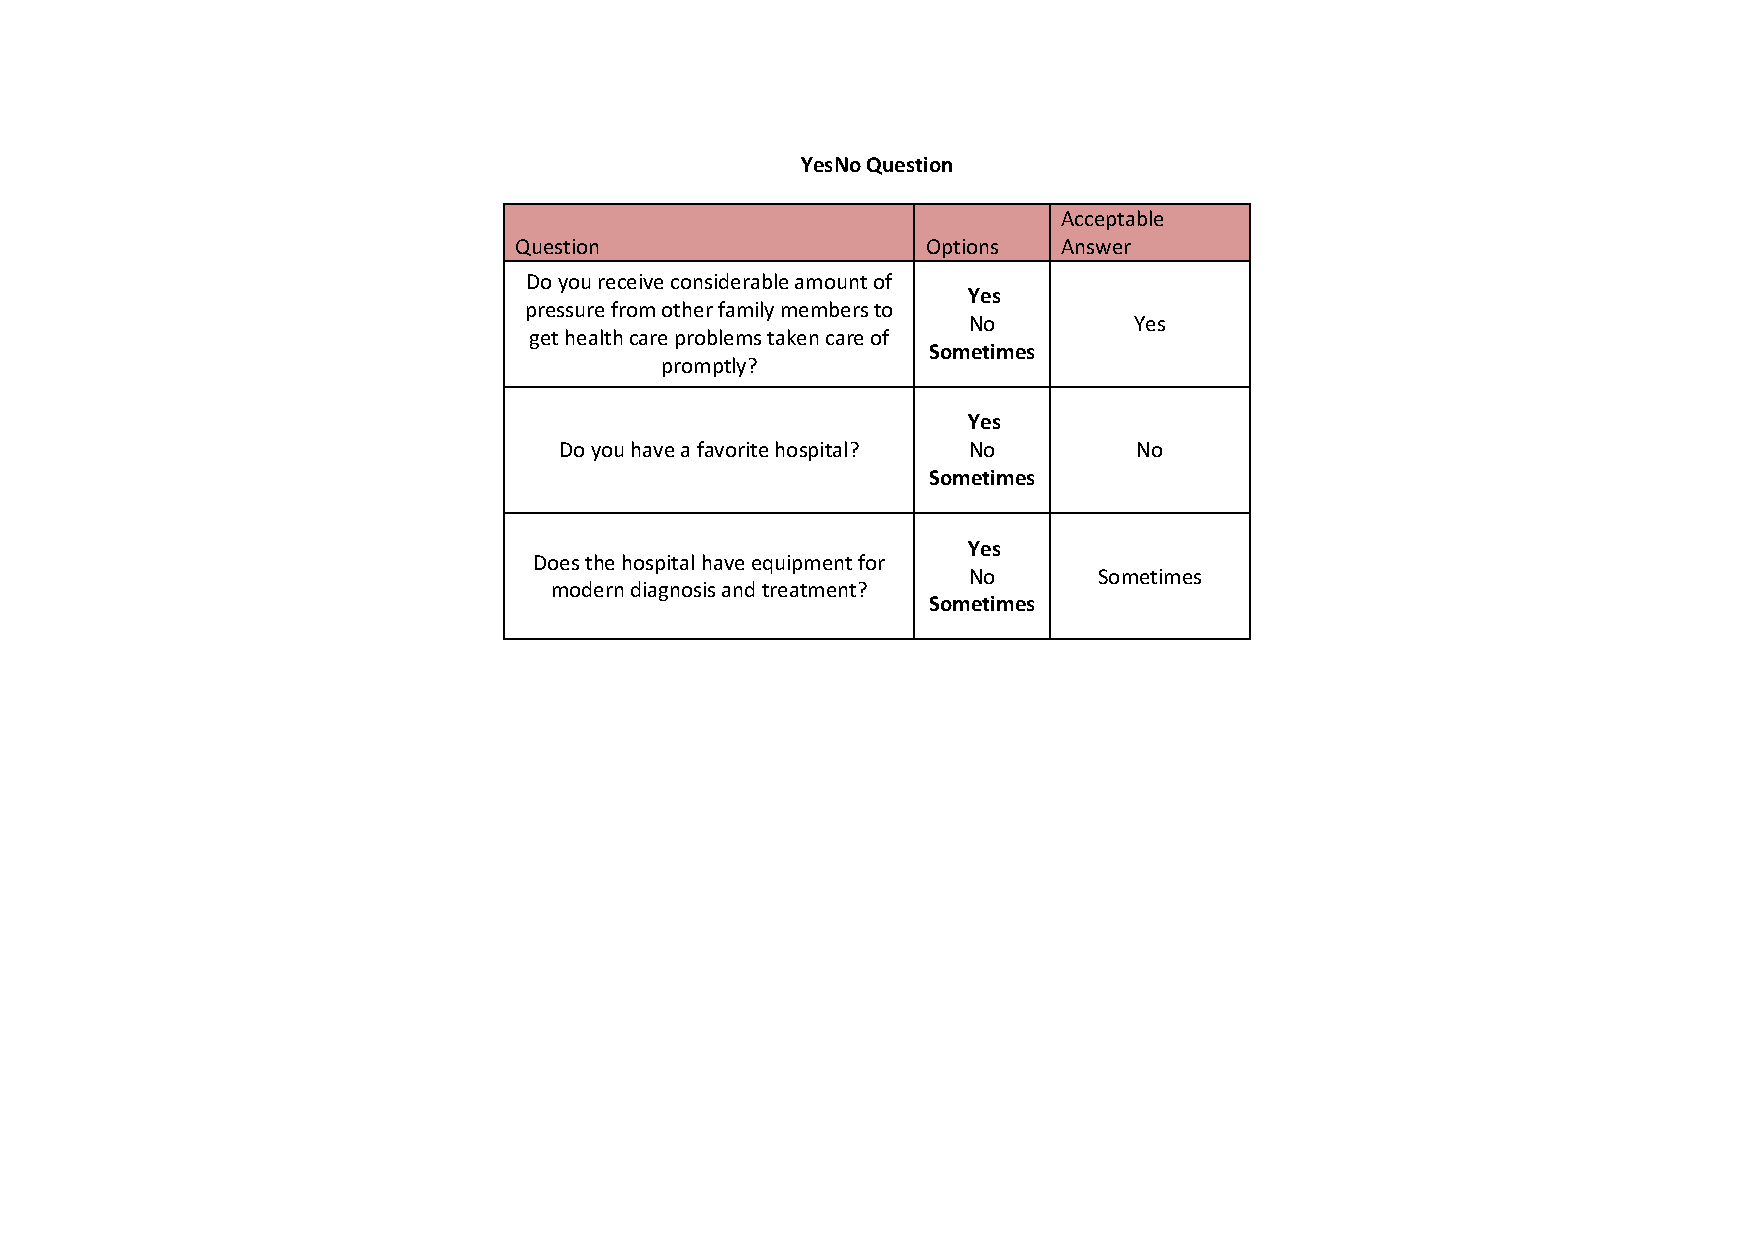
\includepdf[pages=-,pagecommand={\pagestyle{fancy}}]{./Specs/1.pdf}

\begin{figure}[H]
	\center{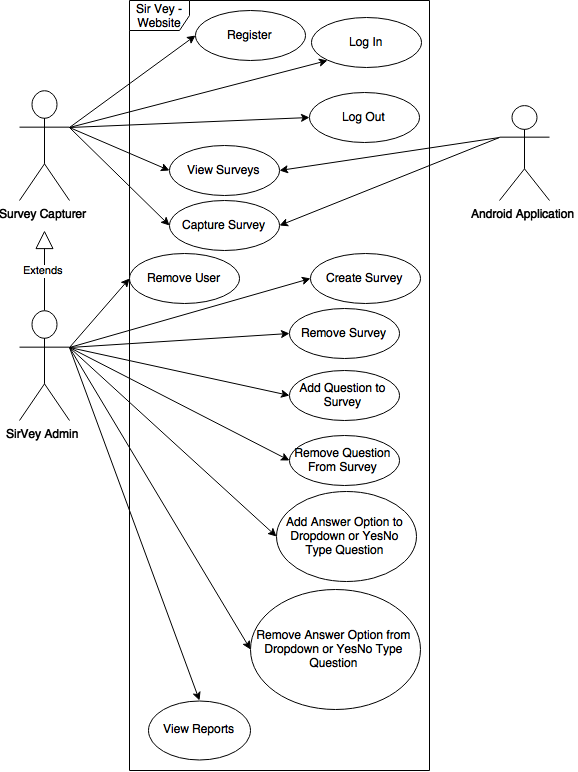
\includegraphics[width=.95\linewidth]{./images/SirVeyUMLDiagram.png}} 
	\caption{Use Case Diagram for SirVey Application.} 
	\label{fig:UseCase}
\end{figure}

\newpage
\section{Appendix C: Sprint Planning}
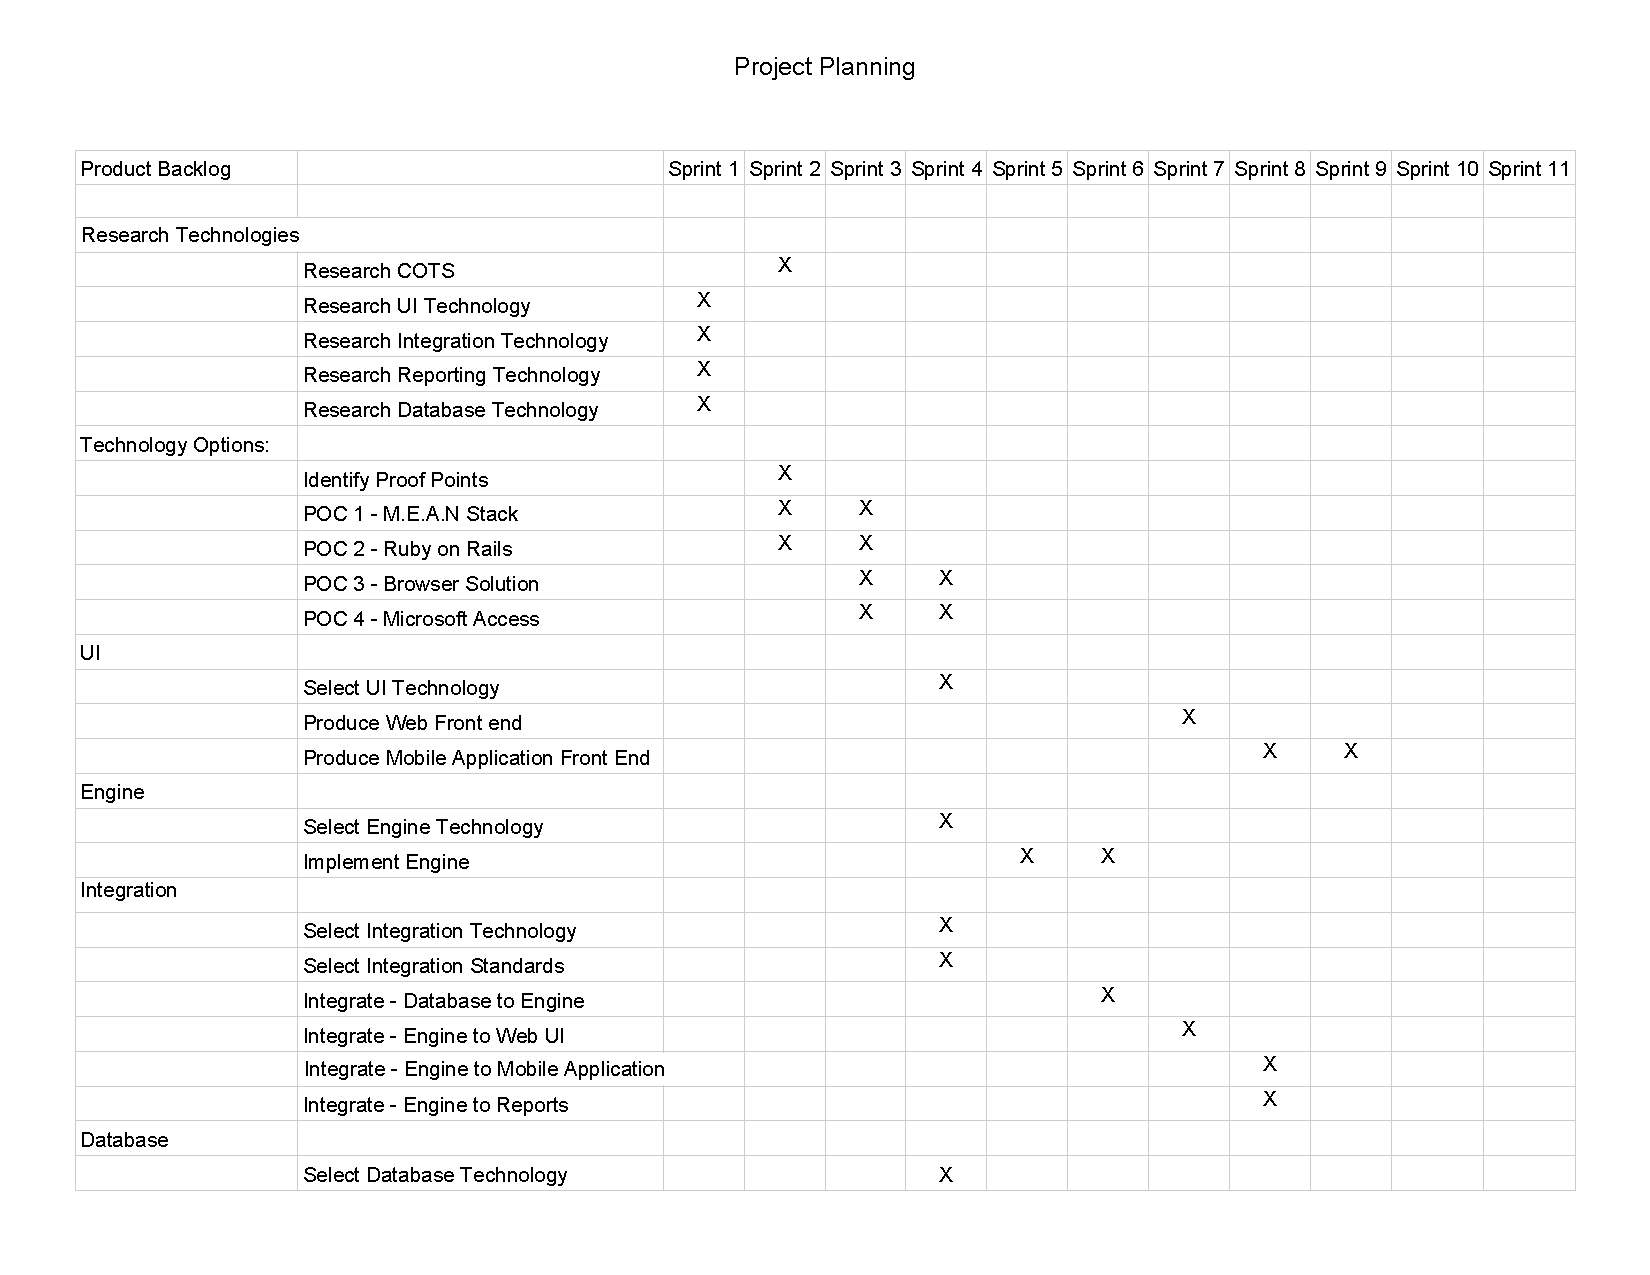
\includepdf[pages=-,pagecommand={\pagestyle{fancy}}]{./sprint_planning/ProjectPlanning.pdf}


\newpage
\section{Appendix D: Developer Guide}
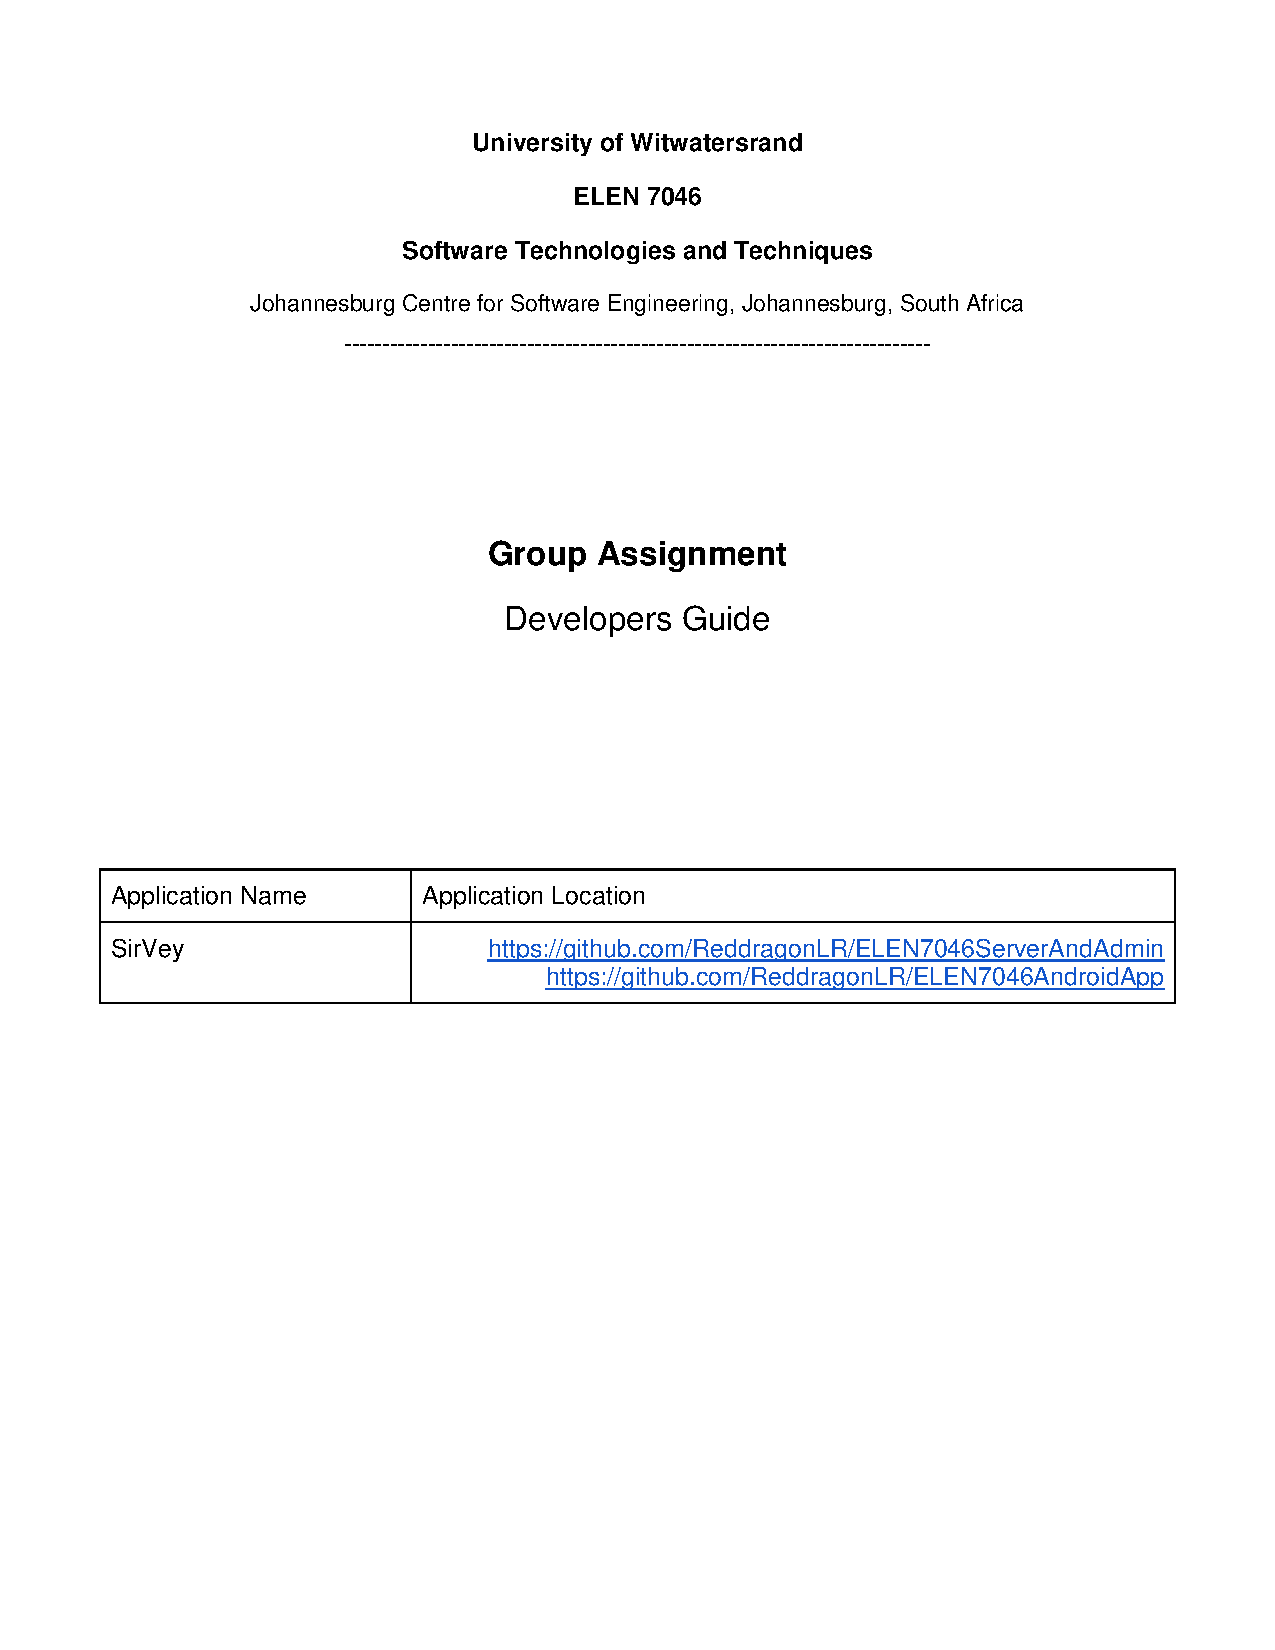
\includepdf[pages=-,pagecommand={\pagestyle{fancy}}]{./Guides/DevelopersGuide.pdf}

\newpage
\section{Appendix E: User Training Guide}

\includepdf[pages=-,pagecommand={\pagestyle{fancy}}]{./Guides/UserGuide.pdf}

\newpage
\section{Appendix F: Final prototype Reports}
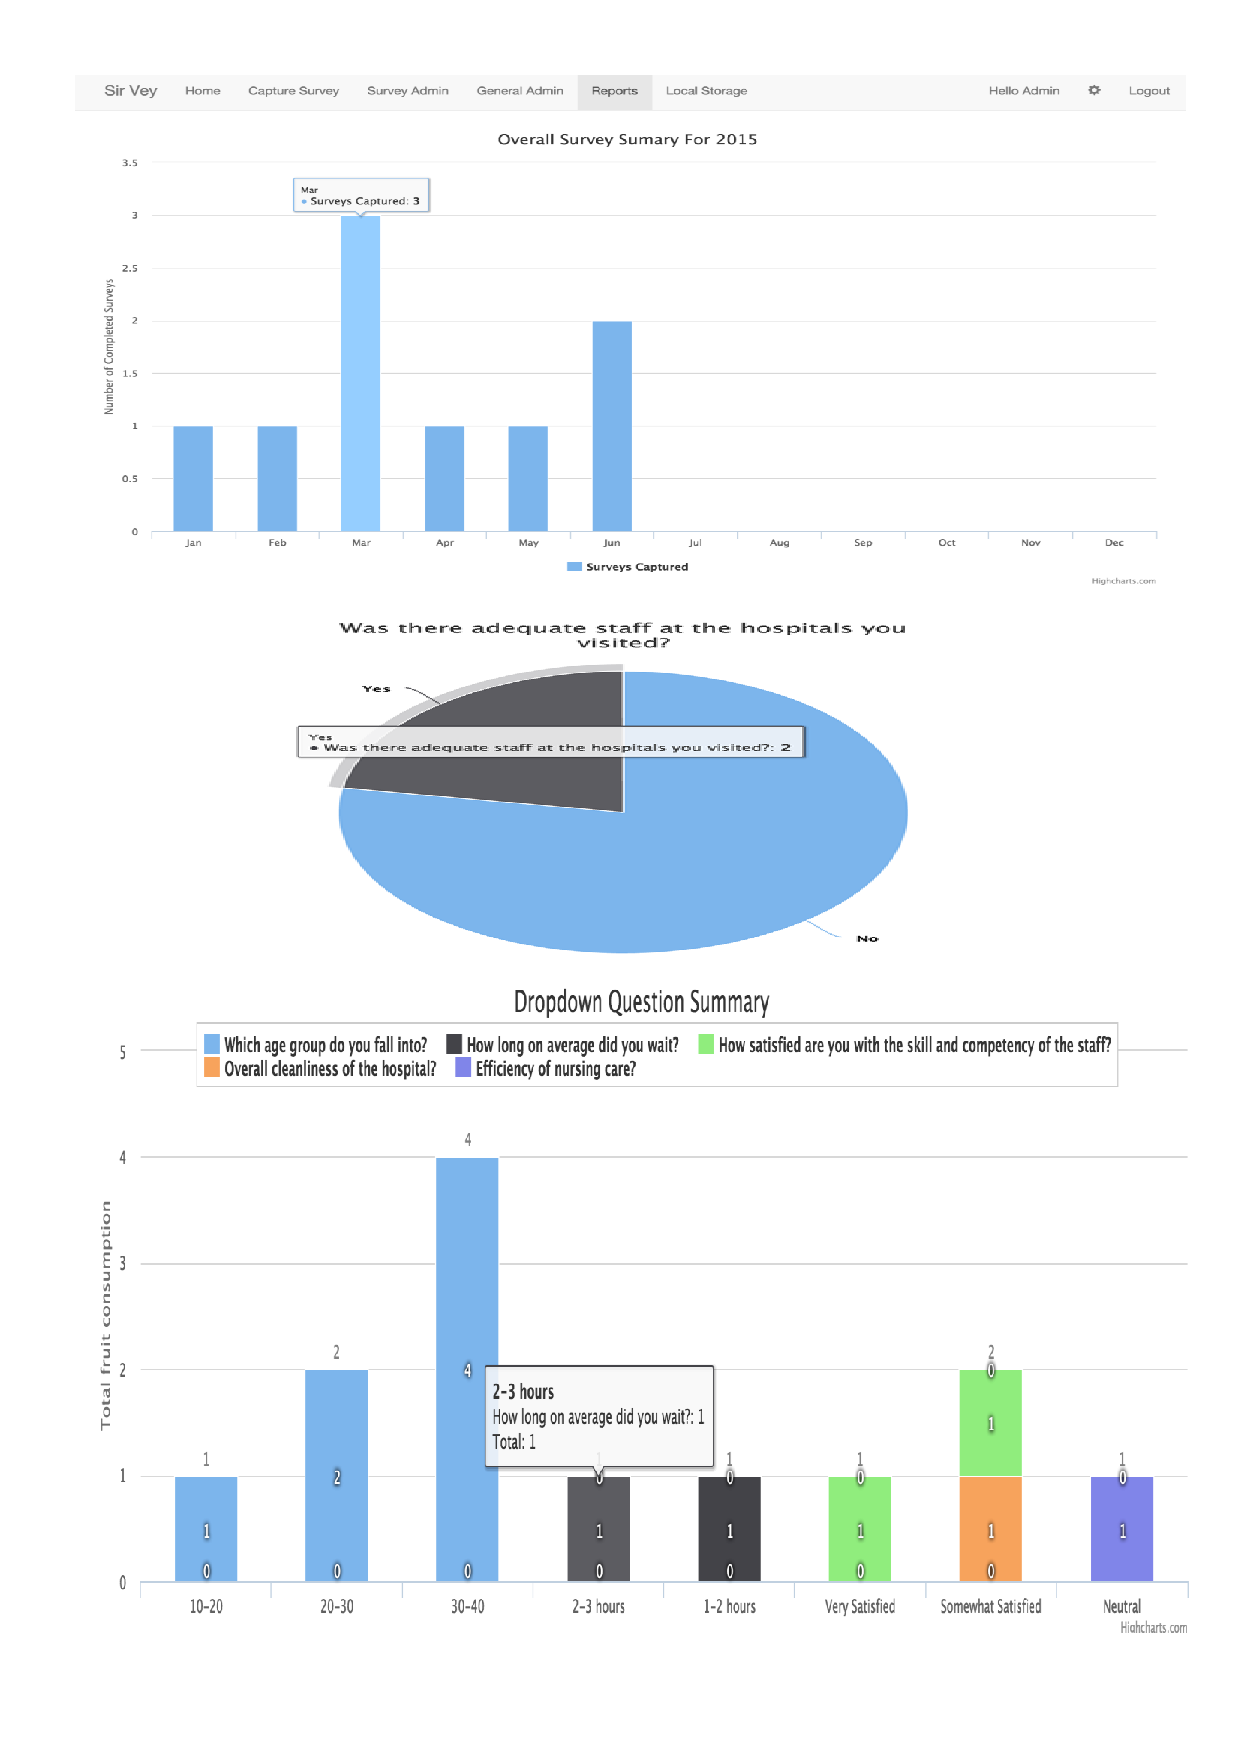
\includepdf[pages=-,pagecommand={\pagestyle{fancy}}]{./Guides/FinalReports.pdf}

\newpage
\section{Appendix H: Group Timesheet}
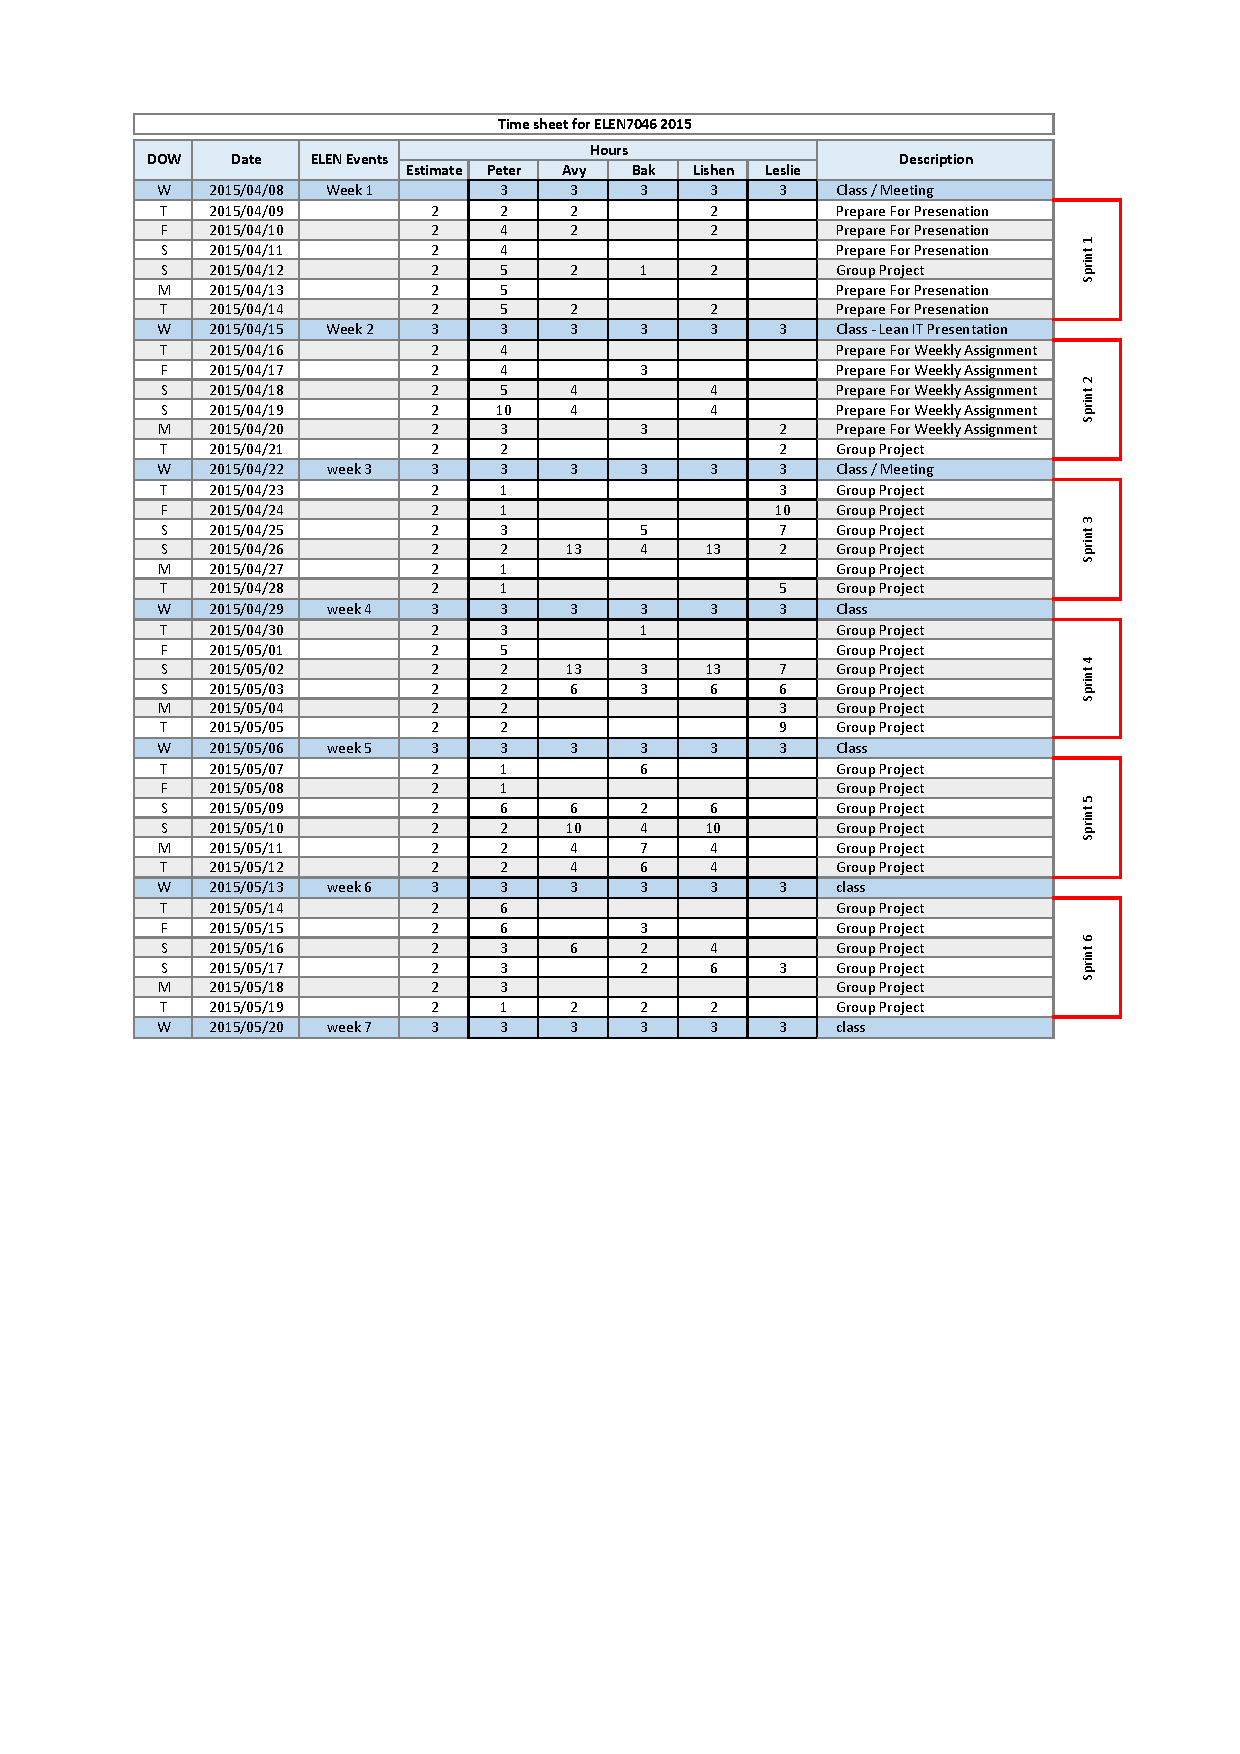
\includepdf[pages=-,pagecommand={\pagestyle{fancy}}]{./Guides/GroupTimeSheet.pdf}

\newpage
\section{Appendix I: MIT License}
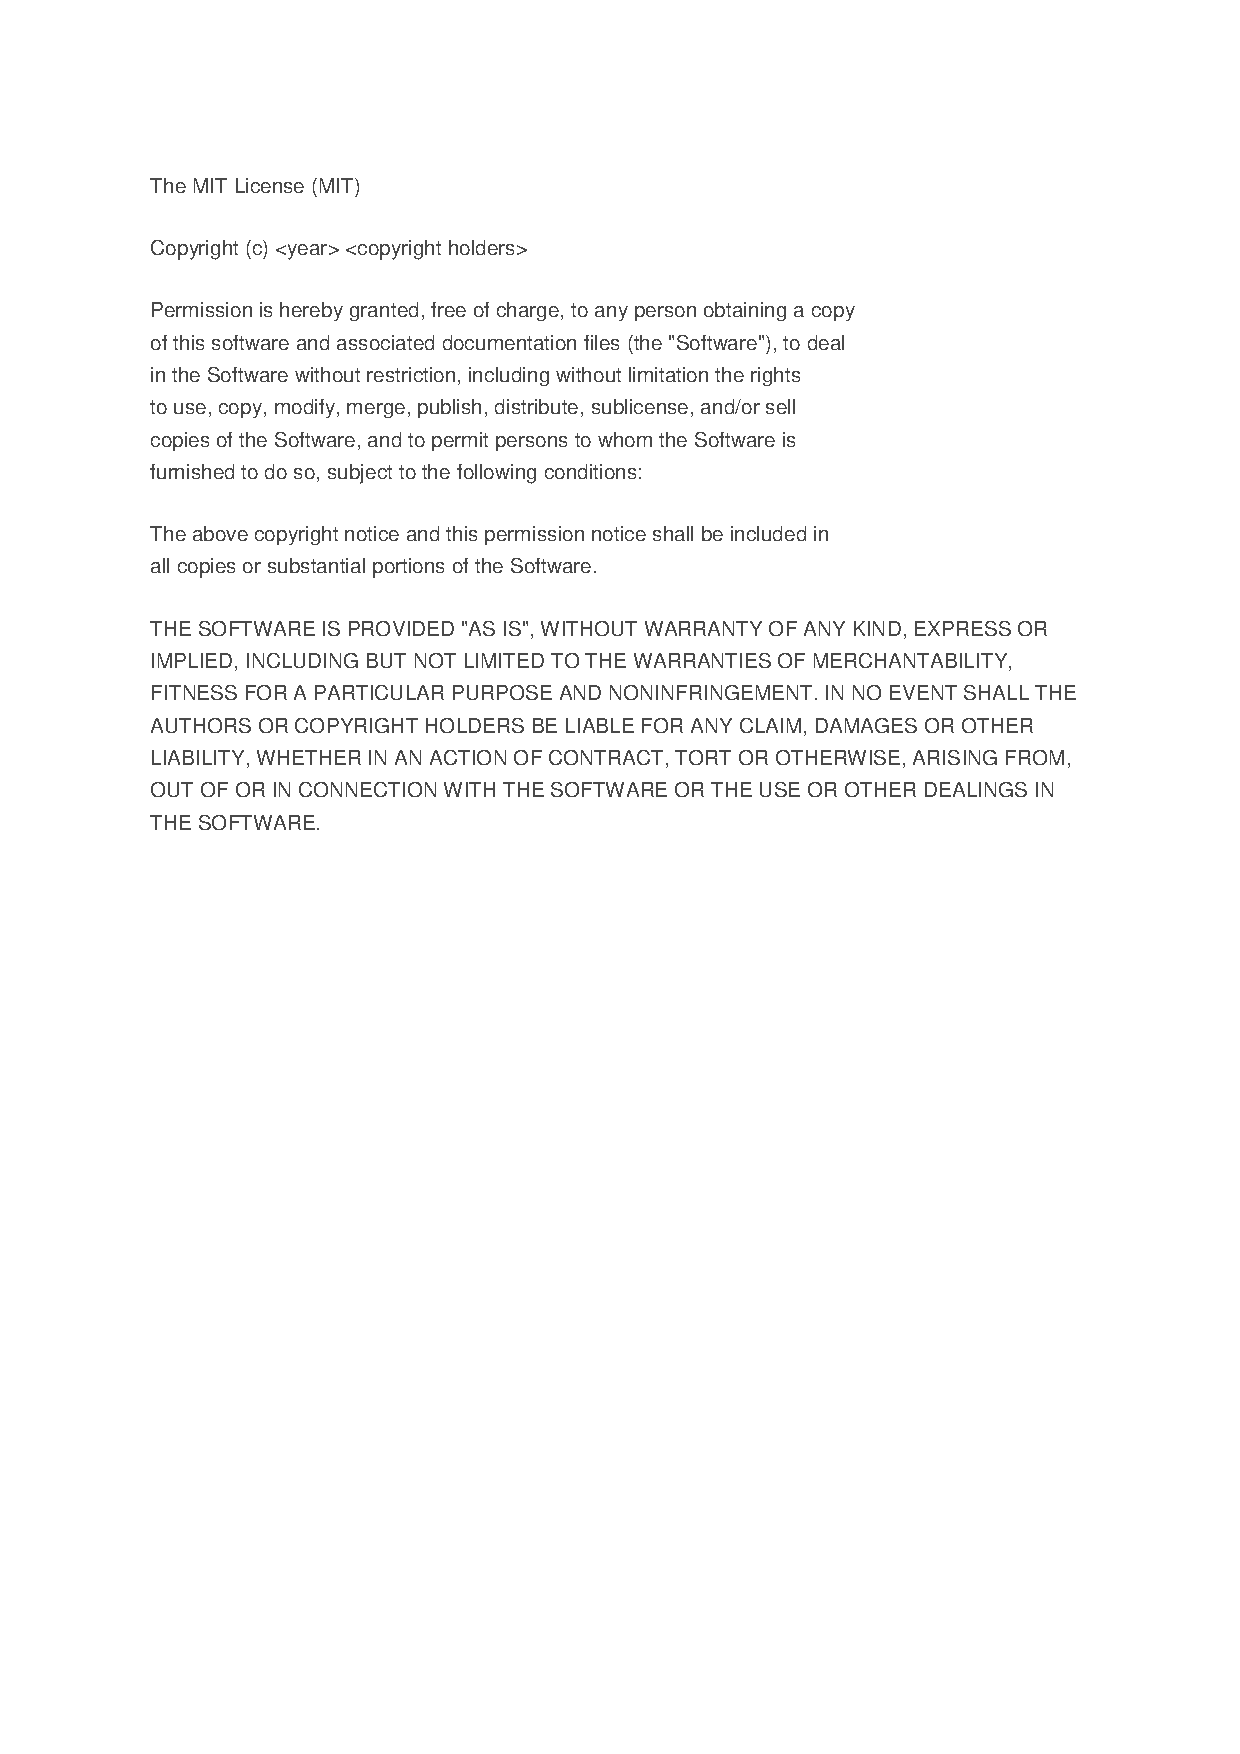
\includepdf[pages=-,pagecommand={\pagestyle{fancy}}]{./Guides/MIT.pdf}

\end{document}

% Appendix

%   A - Requirements Engineering Documentation 
% 	B - Use case diagrams
%   C - Sprint Planning / Project Planning
%   D - Dev User Guide
%   E - User Training Guide
%   F - Report Demo / Example
%   G - Meeting Minutes
%   H - Group Timesheets
%   I - Licenses
